%%%%%%%%%%%%%%%%%%%%%%%%%%%%%%%%%%%%%%%%%%%%%%%%%%%%%%%%%%%%%%%%%%%%%%%%%%%%%%%%%%
\begin{frame}[fragile]\frametitle{}
\begin{center}
{\Large Introduction to LangGraph}
\end{center}
\end{frame}

%%%%%%%%%%%%%%%%%%%%%%%%%%%%%%%%%%%%%%%%%%%%%%%%%%%%%%%%%%%%%%%%%%%%%%%%%%%%%%%%%%
\begin{frame}\frametitle{What is LangGraph?}

\begin{itemize}
\item Building state-ful multi agent applications using LLMs (Large Language Models)
\item So, components are not in `chain' as in LangChain (ie Sequential) but can a Graph.
\item Like Workflow modeling or orchestration
\end{itemize}

\begin{center}
\includegraphics[width=0.8\linewidth,keepaspectratio]{langgraph1}
\end{center}	  


{\tiny (Ref: Introduction to LangGraph | Building an AI Generated Podcast - Prompt Circle AI)}
\end{frame}

%%%%%%%%%%%%%%%%%%%%%%%%%%%%%%%%%%%%%%%%%%%%%%%%%%%%%%%%%%%
\begin{frame}[fragile]\frametitle{Introduction to LangGraph}
      \begin{itemize}
        \item LangGraph is a graph-based framework for building complex LLM applications
        \item Represents AI workflows as directed graphs with nodes, edges, and data states
        \item Addresses limitations of LCEL and AgentExecutor in complex scenarios
        \item Provides intuitive and flexible approach to constructing conversational flows
        \item Supports looping, branching, and dynamic execution paths
        \item Enables state persistence and human-machine interaction
        \item Seamlessly integrates with existing LangChain ecosystem
        \item Offers streaming processing and real-time feedback capabilities
      \end{itemize}
\end{frame}

%%%%%%%%%%%%%%%%%%%%%%%%%%%%%%%%%%%%%%%%%%%%%%%%%%%%%%%%%%%
\begin{frame}[fragile]\frametitle{Limitations of LCEL Chain Expressions}
      \begin{itemize}
        \item Linear processes with predefined execution order
        \item Difficulty in dynamic routing and conditional branching
        \item Complex state management in multi-turn conversations
        \item Manual state passing and updates increase code complexity
        \item Non-intuitive tool integration and coordination
        \item Nested tools create highly complex LCEL expressions
        \item Limited flexibility for dynamic conversational scenarios
        \item Error-prone state management across chain calls
      \end{itemize}
\end{frame}

%%%%%%%%%%%%%%%%%%%%%%%%%%%%%%%%%%%%%%%%%%%%%%%%%%%%%%%%%%%
\begin{frame}[fragile]\frametitle{LCEL Complexity Example}
      \begin{lstlisting}[language=Python, basicstyle=\tiny]
# Decomposition chain
decomposition_chain = (
    {"question": RunnablePassthrough()}
    | decomposition_prompt
    | ChatOpenAI(model="gpt-4o-mini", temperature=0)
    | StrOutputParser()
    | (lambda x: x.strip().split("\n"))
)

# Sub-question answer generation chain
sub_question_chain = (
    {"context": retriever, "question": RunnablePassthrough()}
    | sub_question_prompt
    | ChatOpenAI(model="gpt-4o-mini")
    | StrOutputParser()
)

# Assembly chain
chain = (
    {"question": RunnablePassthrough(), "context": decomposition_chain}
    | {"questions": RunnablePassthrough(), "answers": sub_question_chain.map()}
    | RunnableLambda(format_qa_pairs)
    | prompt
    | llm_output_str
)
      \end{lstlisting}
\end{frame}

%%%%%%%%%%%%%%%%%%%%%%%%%%%%%%%%%%%%%%%%%%%%%%%%%%%%%%%%%%%
\begin{frame}[fragile]\frametitle{Limitations of AgentExecutor}
      \begin{itemize}
        \item Complex configuration for conversational flows and multi-turn dialogues
        \item Limited dynamic routing capability for conditional branches
        \item Lack of built-in state persistence mechanism
        \item Over-encapsulation with fixed input requirements
        \item Black-box uncontrollability in tool usage order
        \item Cannot insert human interaction during execution
        \item Difficult secondary development due to rigid structure
        \item Must restart from scratch when conversation resumes
      \end{itemize}
\end{frame}


% %%%%%%%%%%%%%%%%%%%%%%%%%%%%%%%%%%%%%%%%%%%%%%%%%%%%%%%%%%%%%%%%%%%%%%%%%%%%%%%%%%
% \begin{frame}[fragile]\frametitle{Why LangGraph?}

% \begin{itemize}
% \item Most of the Multi-agent frameworks are rigid, monolithic
% \item LangGraph decouples the agents from their orchestration.
% \item Here, agents can have different LLMs, can combine even non-LLM services together, can combine agents from other systems such as Autogen or Crew AI etc.
% \end{itemize}


% {\tiny (Ref: Langgraph: The Agent Orchestrator - Rajib Deb)}

% \begin{lstlisting}
% agent_1 = MyAgent("agent_1")
% agent_2 = MyAgent("agent_2")
% group_chat = [agent_1,agent_2]
% group_chat.invoke("What is GST?")
% \end{lstlisting}

% \end{frame}


%%%%%%%%%%%%%%%%%%%%%%%%%%%%%%%%%%%%%%%%%%%%%%%%%%%%%%%%%%%
\begin{frame}[fragile]\frametitle{LangChain vs LangGraph}
\begin{columns}
    \begin{column}[T]{0.6\linewidth}
        \begin{center}
        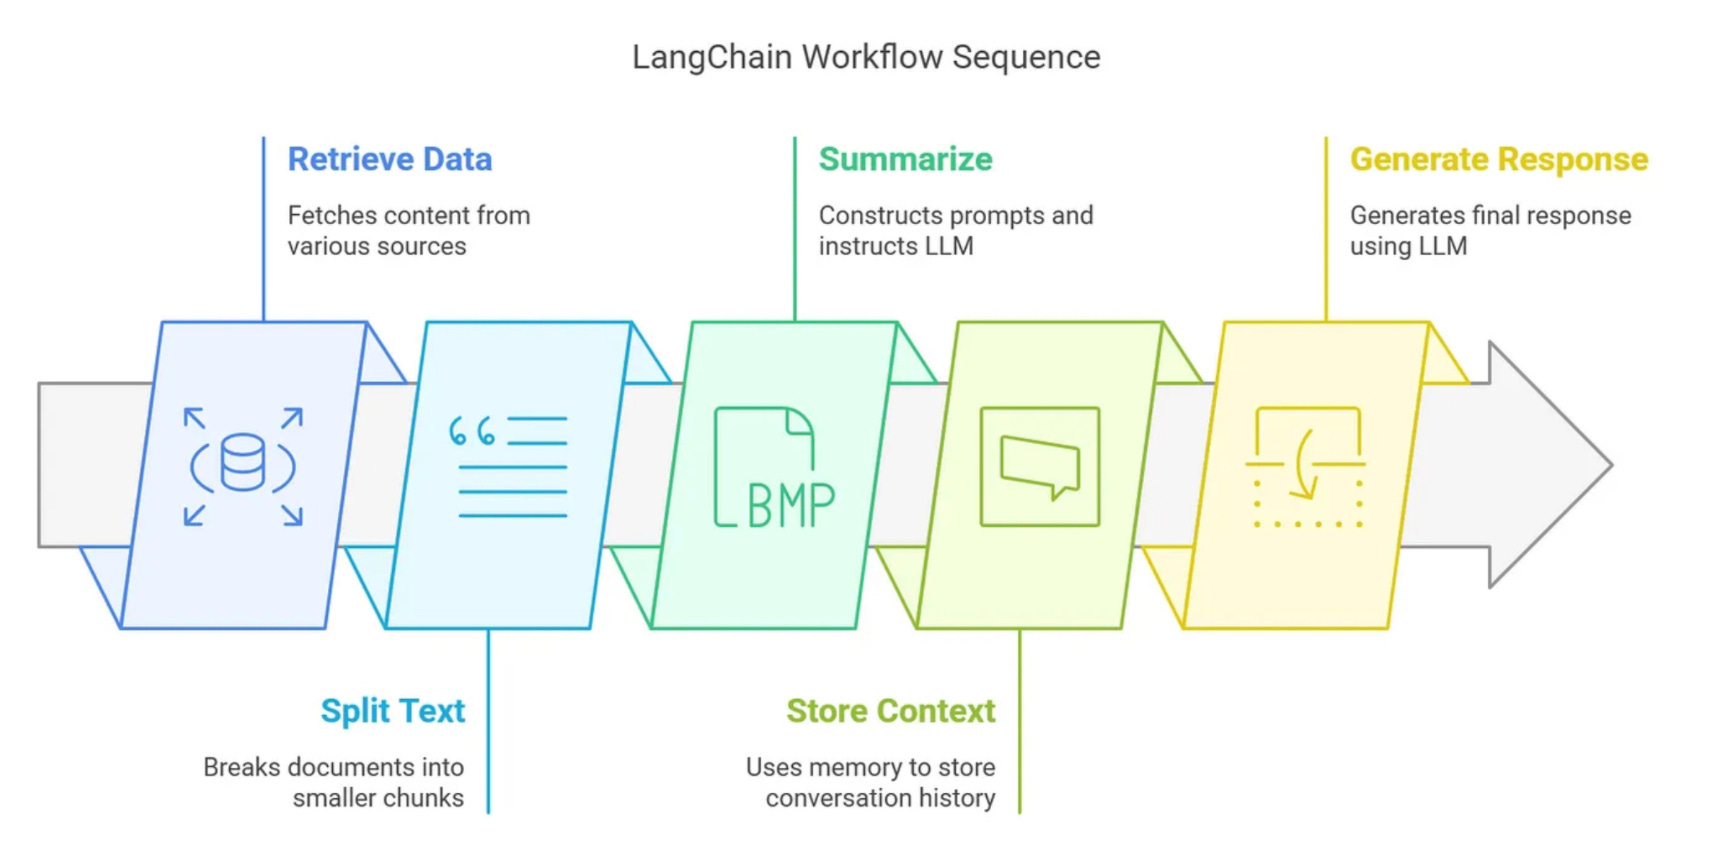
\includegraphics[width=0.8\linewidth,keepaspectratio]{aiagents64}
		
        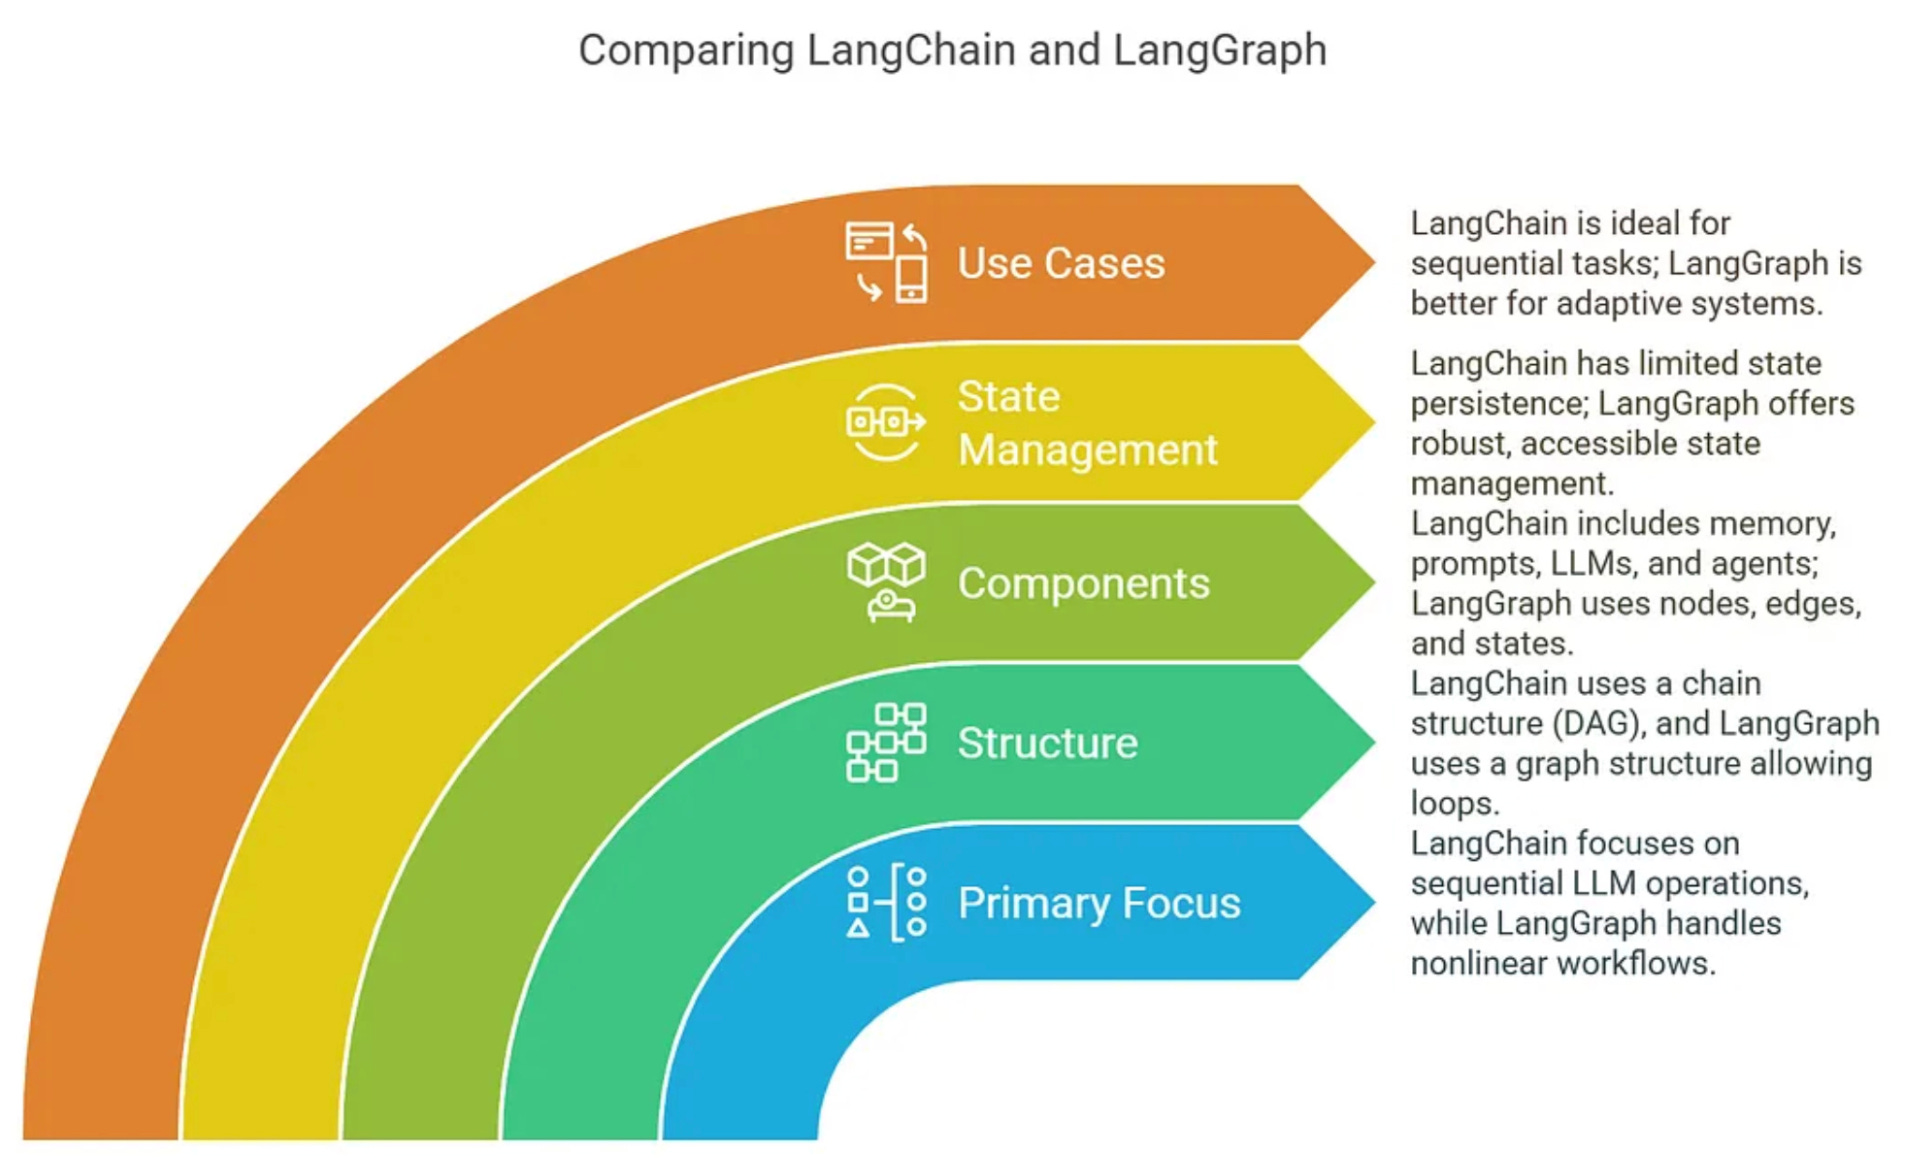
\includegraphics[width=0.8\linewidth,keepaspectratio]{aiagents66}
		
		{\tiny (Ref: Vizuara AI Agents Bootcamp)}
				
        \end{center}    
    \end{column}
    \begin{column}[T]{0.4\linewidth}
        \begin{center}
        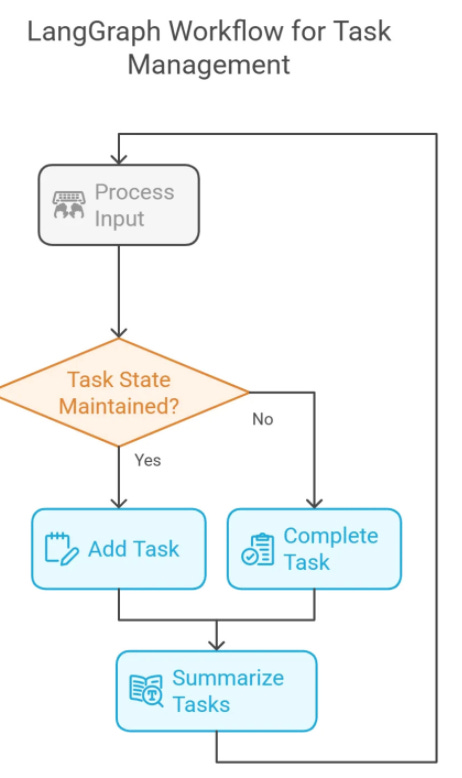
\includegraphics[width=0.8\linewidth,keepaspectratio]{aiagents65}
		
		{\tiny (Ref: Vizuara AI Agents Bootcamp)}
				
        \end{center}    
    \end{column}
  \end{columns}
\end{frame}


%%%%%%%%%%%%%%%%%%%%%%%%%%%%%%%%%%%%%%%%%%%%%%%%%%%%%%%%%%%
\begin{frame}[fragile]\frametitle{LangChain vs LangGraph – Why a New Approach?}

      \begin{itemize}
        \item LangChain excels at straightforward pipelines with fixed sequential tasks (retrieve → summarize → answer)
        \item Real-world workflows aren't always linear - they need branches, loops, and dynamic decision points
        \item LangGraph specializes in stateful, non-linear workflows within the LangChain ecosystem
        \item LangGraph exposes control flow explicitly, allowing fine-grained control over agent behavior
        \item You define a graph of possible steps instead of a rigid chain structure
        \item Agents can revisit nodes or choose different paths dynamically based on conditions
        \item Use LangChain for simple sequences, LangGraph for conditional logic and extended context
        \item LangGraph enables complex multi-agent systems with evolving task flows
      \end{itemize}

\end{frame}

%%%%%%%%%%%%%%%%%%%%%%%%%%%%%%%%%%%%%%%%%%%%%%%%%%%%%%%%%%%
\begin{frame}[fragile]\frametitle{LangGraph Fundamentals: Nodes, Edges \& State}

      \begin{itemize}
        \item \textbf{Nodes (N):} Individual processing steps implemented as Python functions that transform state
        \item Each node encapsulates one sub-task: LLM calls, calculations, file operations, or tool invocations
        \item \textbf{Edges (E):} Directed connections determining execution order and flow between nodes
        \item Edges can be linear progressions or conditional routes based on current state
        \item \textbf{State (S):} Shared data object (dictionary/TypedDict) persisting throughout agent execution
        \item State enables context and memory across workflow, allowing nodes to read previous results
        \item StateGraph ties everything together with designated START and END nodes
        \item This approach handles interactive, conditional loops that static chains struggle with
      \end{itemize}
  

\end{frame}

%%%%%%%%%%%%%%%%%%%%%%%%%%%%%%%%%%%%%%%%%%%%%%%%%%%%%%%%%%%
\begin{frame}[fragile]\frametitle{LangGraph}
\begin{columns}
    \begin{column}[T]{0.5\linewidth}
        \begin{center}
		
        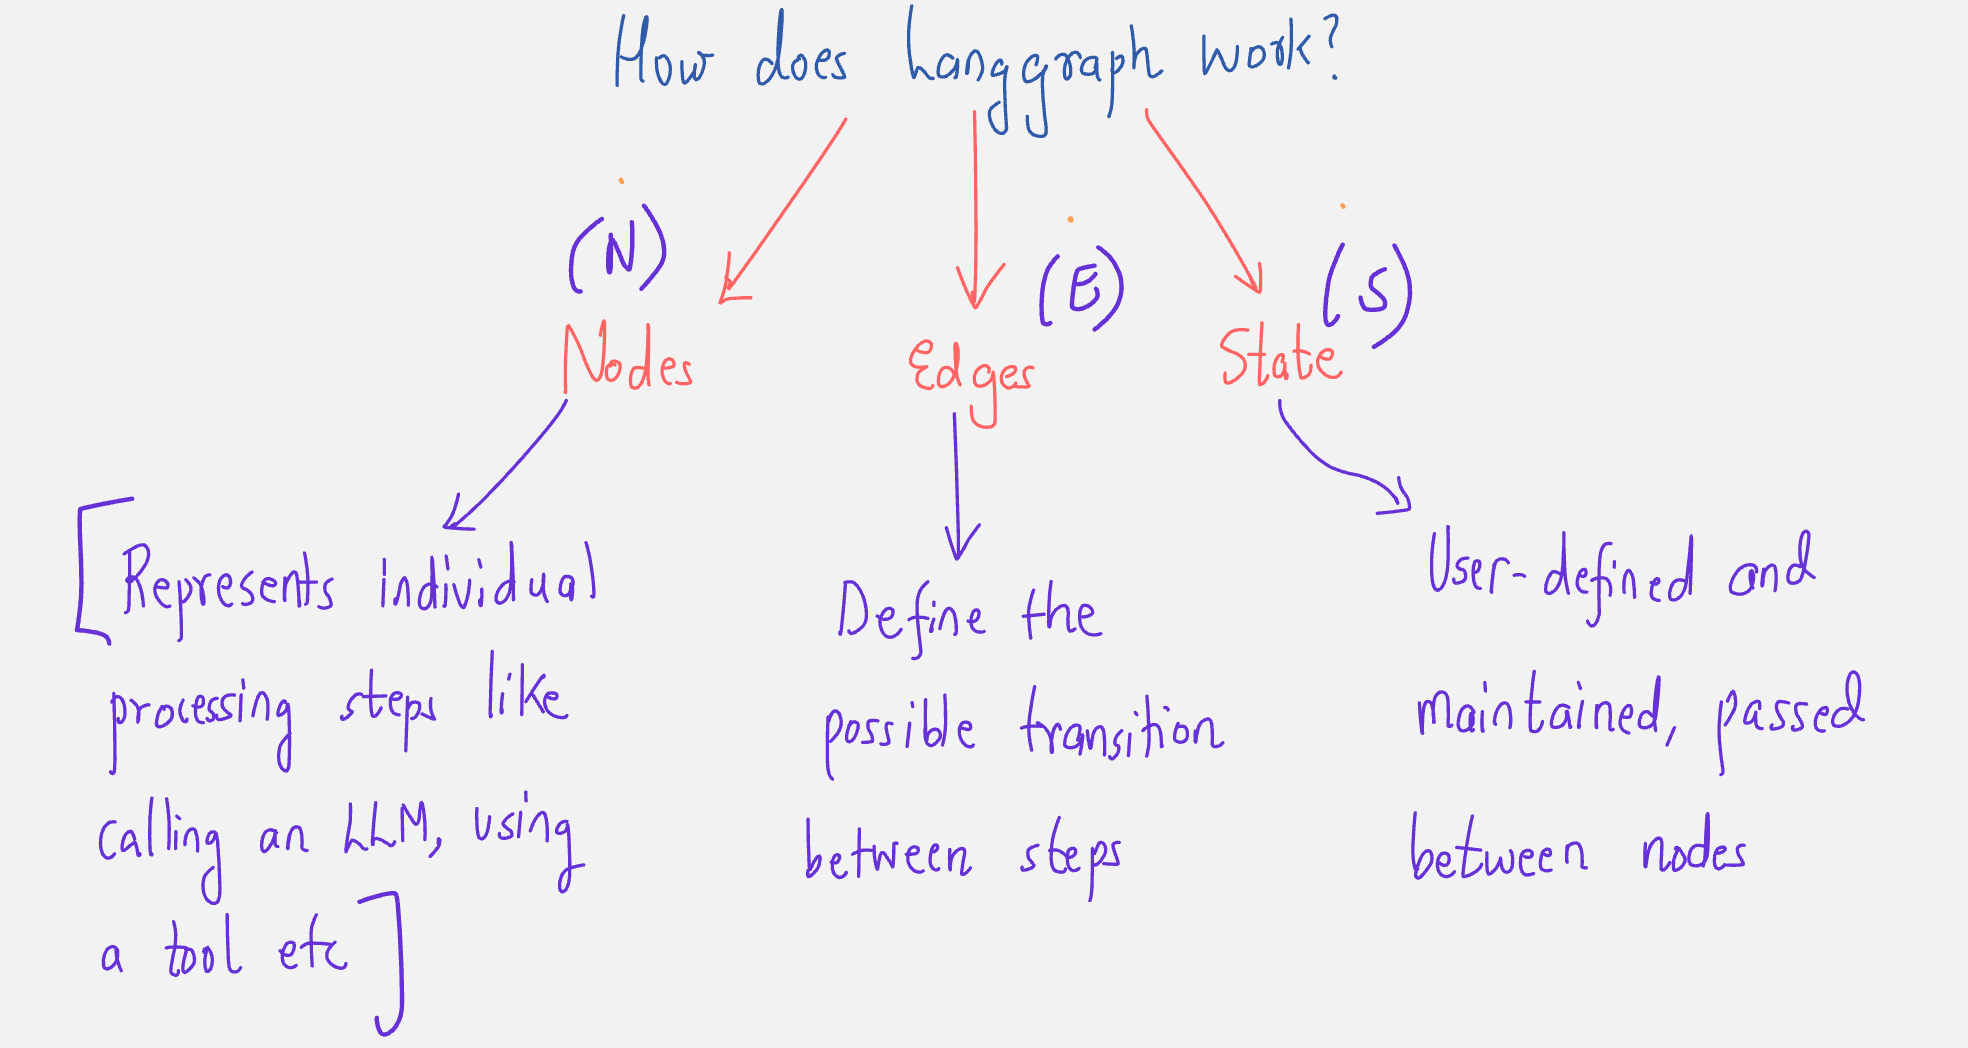
\includegraphics[width=0.8\linewidth,keepaspectratio]{aiagents67}
		
        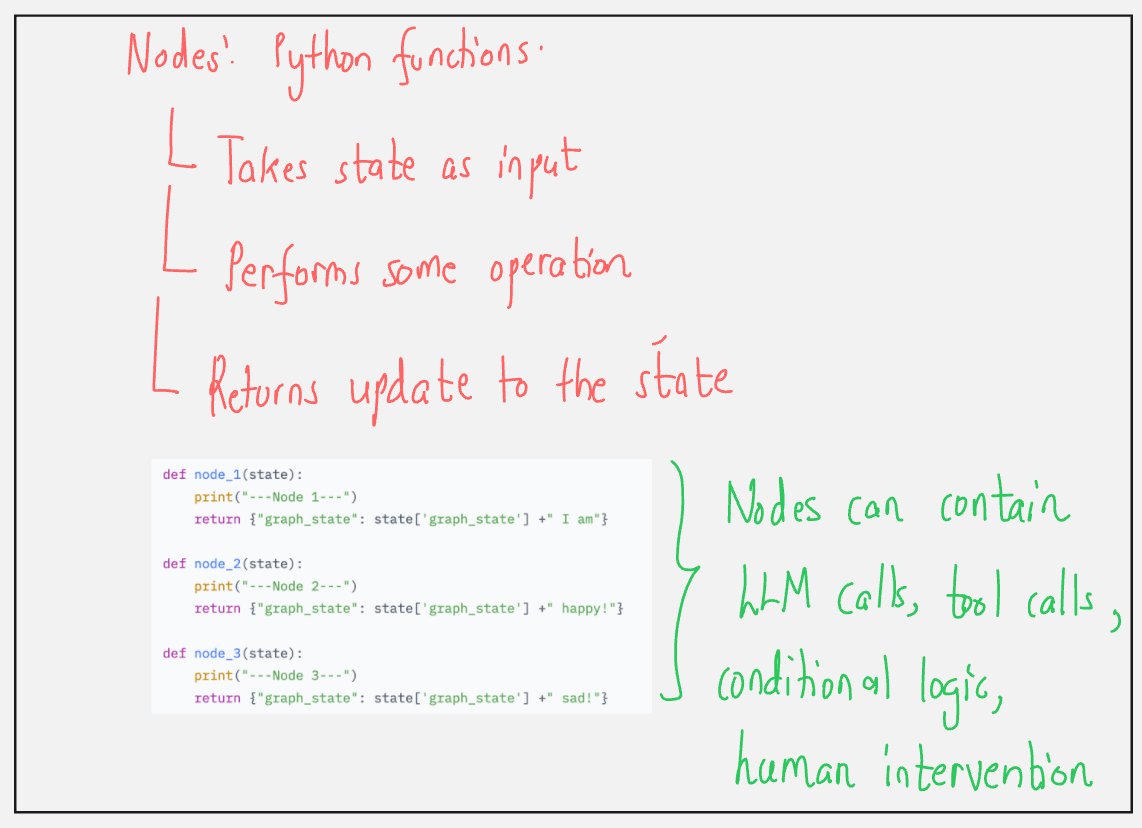
\includegraphics[width=0.8\linewidth,keepaspectratio]{aiagents68}
		
		
		{\tiny (Ref: Vizuara AI Agents Bootcamp)}
				
        \end{center}    
    \end{column}
    \begin{column}[T]{0.5\linewidth}
        \begin{center}
        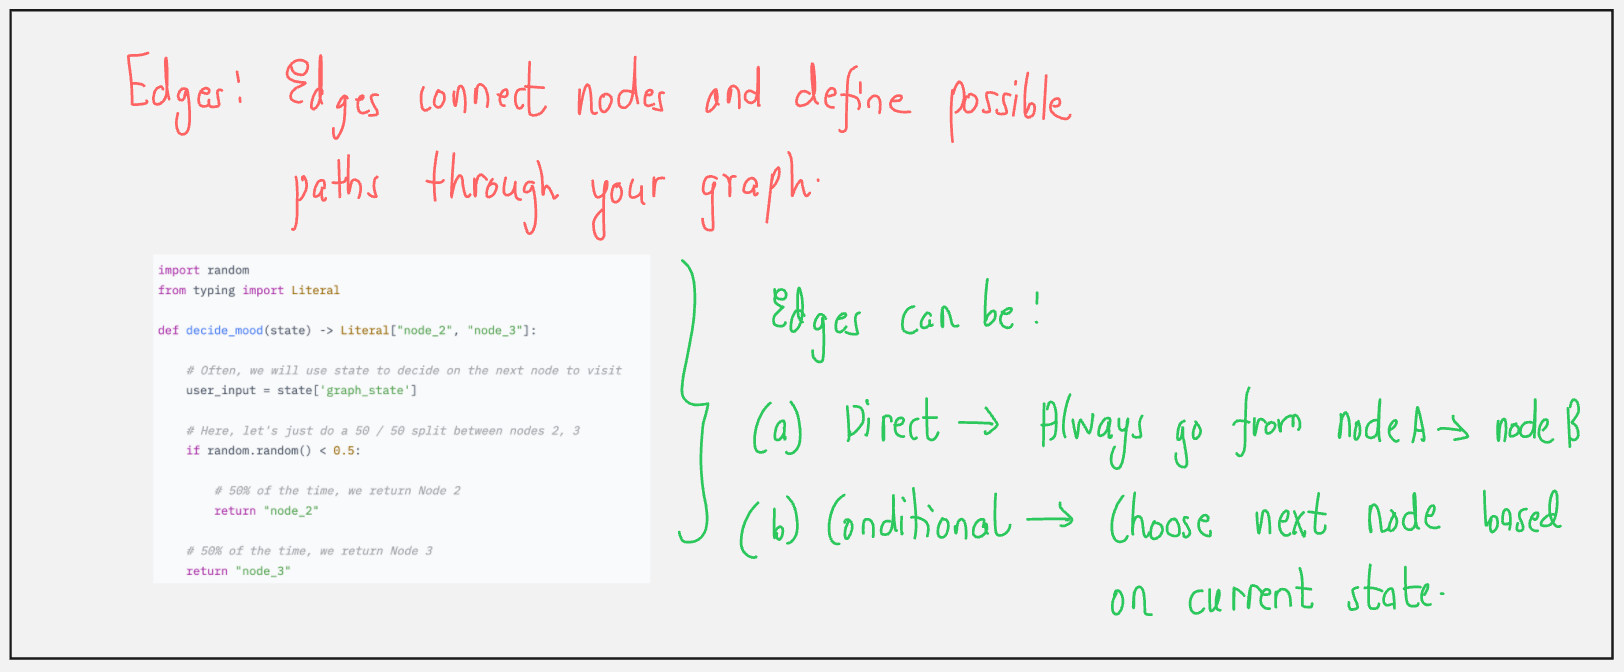
\includegraphics[width=0.8\linewidth,keepaspectratio]{aiagents69}
		
        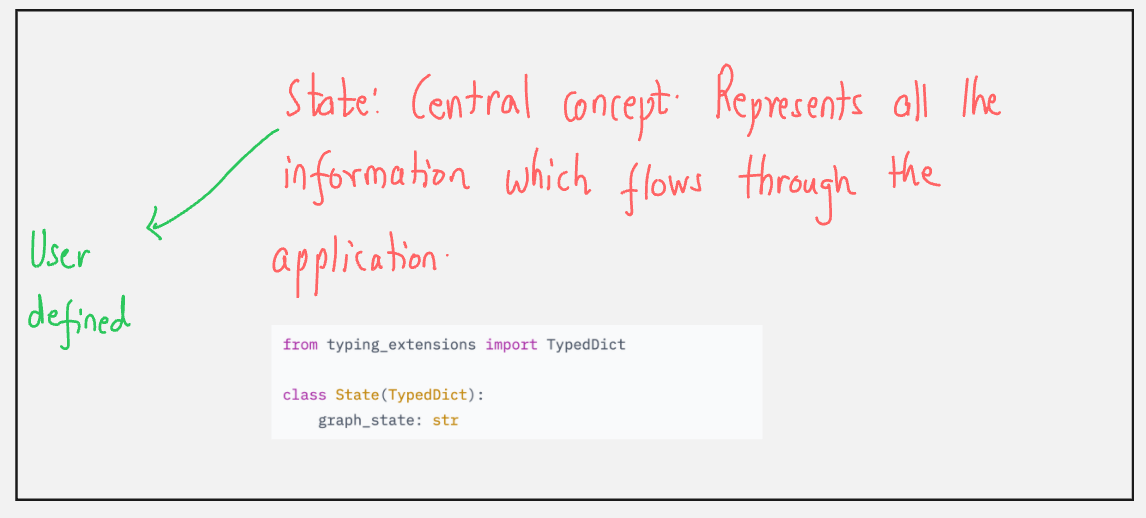
\includegraphics[width=0.8\linewidth,keepaspectratio]{aiagents70}
		
        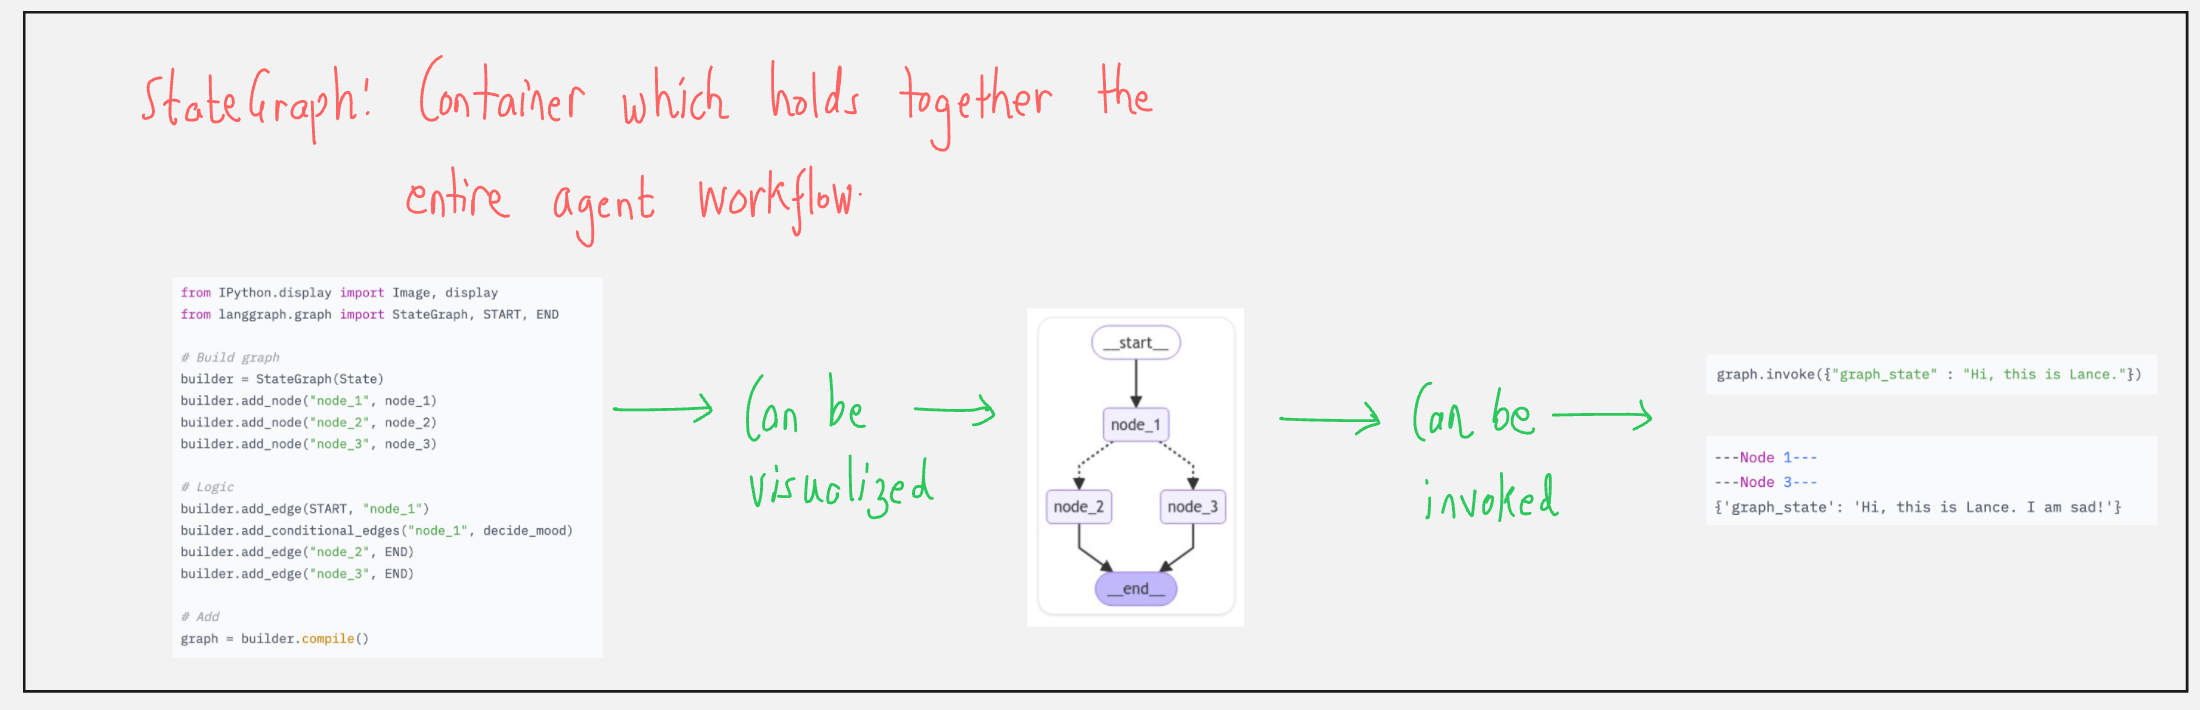
\includegraphics[width=0.8\linewidth,keepaspectratio]{aiagents71}
		
		{\tiny (Ref: Vizuara AI Agents Bootcamp)}
				
        \end{center}    
    \end{column}
  \end{columns}
\end{frame}

%%%%%%%%%%%%%%%%%%%%%%%%%%%%%%%%%%%%%%%%%%%%%%%%%%%%%%%%%%%
\begin{frame}[fragile]\frametitle{Building an Email Sorting Agent}

      \begin{itemize}
        \item Email processing assistant inspired by Alfred managing Bruce Wayne's inbox
        \item \textbf{EmailState:} Contains email content, spam flag, category, draft response, and message history
        \item \textbf{Five nodes:} read\_email → classify\_email → handle\_spam/drafting\_response → notify\_mr\_wayne
        \item Classify\_email uses LLM to analyze content and set spam status in state
        \item Conditional edge routes to spam handler or response drafter based on classification
        \item Handle\_spam terminates workflow early, drafting\_response continues to notification
        \item Demonstrates clear if/else logic through graph structure rather than buried code
        \item Successfully tested on legitimate and crypto spam emails with correct routing
      \end{itemize}

\end{frame}

%%%%%%%%%%%%%%%%%%%%%%%%%%%%%%%%%%%%%%%%%%%%%%%%%%%%%%%%%%%
\begin{frame}[fragile]\frametitle{LangGraph}
\begin{columns}
    \begin{column}[T]{0.5\linewidth}
        \begin{center}
	
        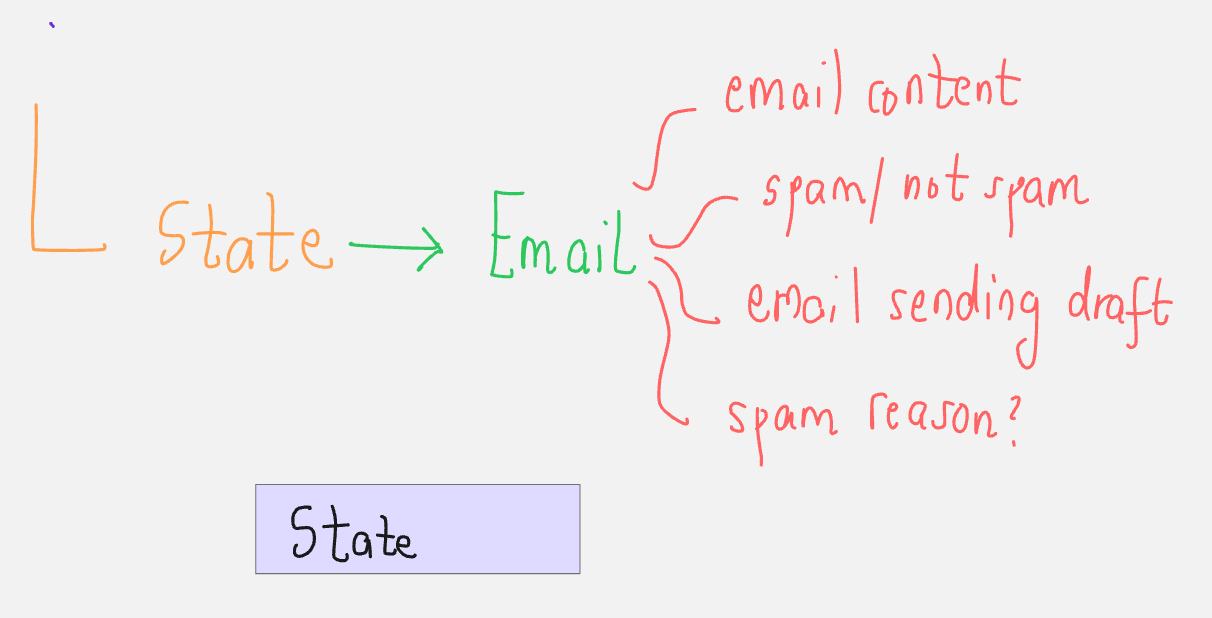
\includegraphics[width=0.8\linewidth,keepaspectratio]{aiagents72}
	
        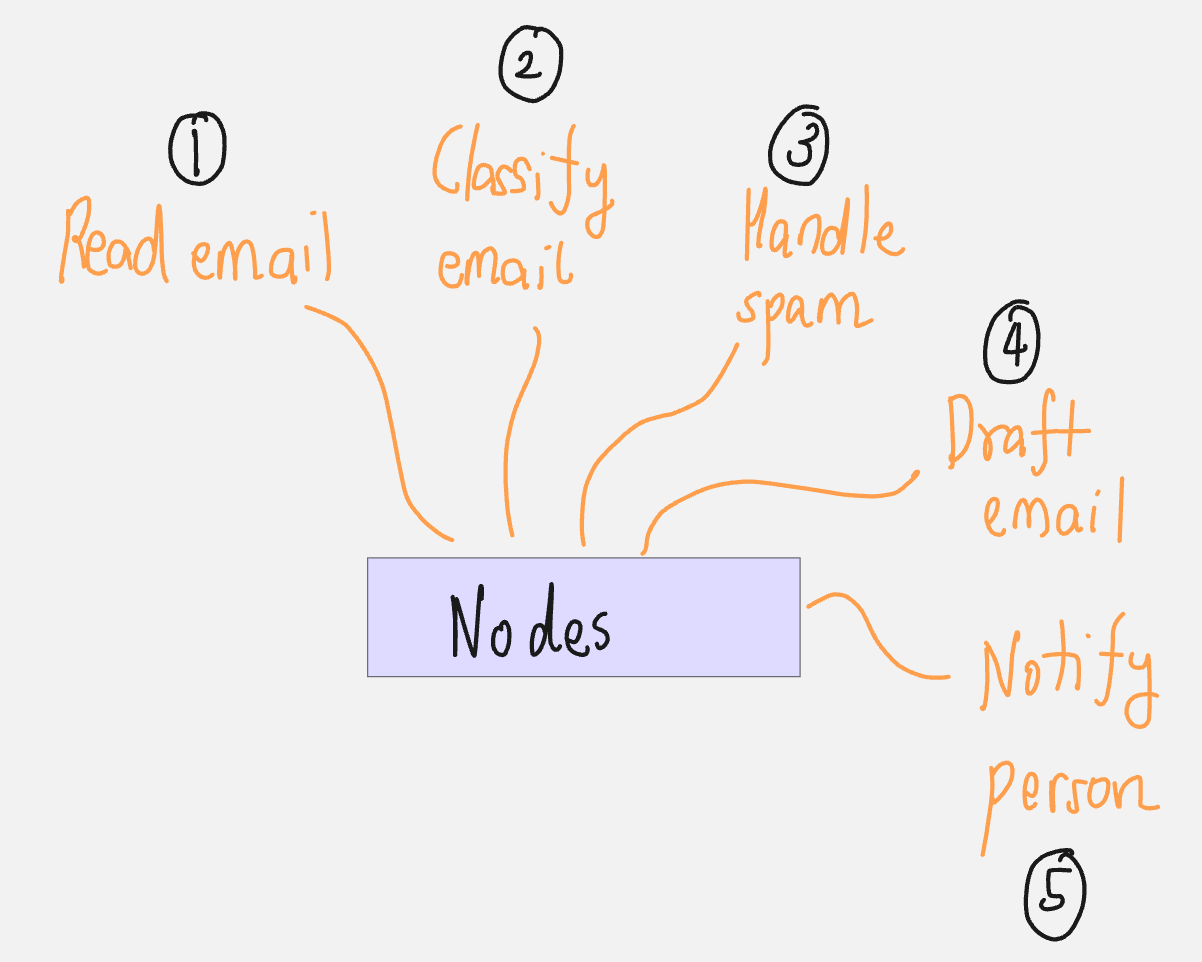
\includegraphics[width=0.8\linewidth,keepaspectratio]{aiagents73}
		
		{\tiny (Ref: Vizuara AI Agents Bootcamp)}
				
        \end{center}    
    \end{column}
    \begin{column}[T]{0.5\linewidth}
        \begin{center}

        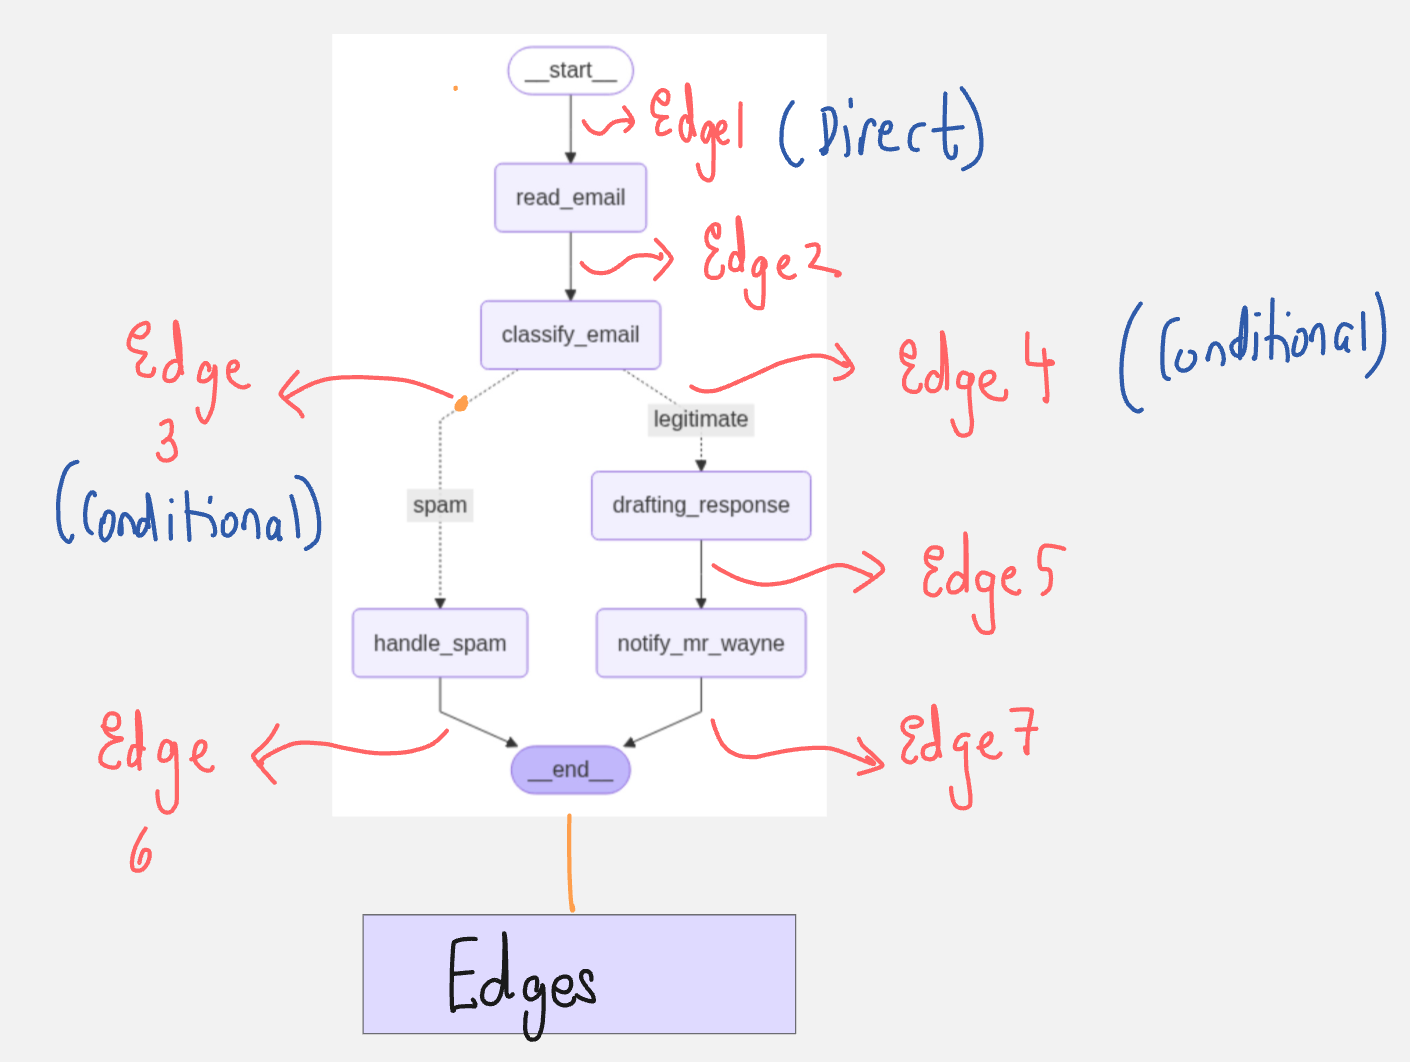
\includegraphics[width=0.8\linewidth,keepaspectratio]{aiagents74}
		
		{\tiny (Ref: Vizuara AI Agents Bootcamp)}
				
        \end{center}    
    \end{column}
  \end{columns}
\end{frame}

%%%%%%%%%%%%%%%%%%%%%%%%%%%%%%%%%%%%%%%%%%%%%%%%%%%%%%%%%%%
\begin{frame}[fragile]\frametitle{LangGraph}

        \begin{center}

        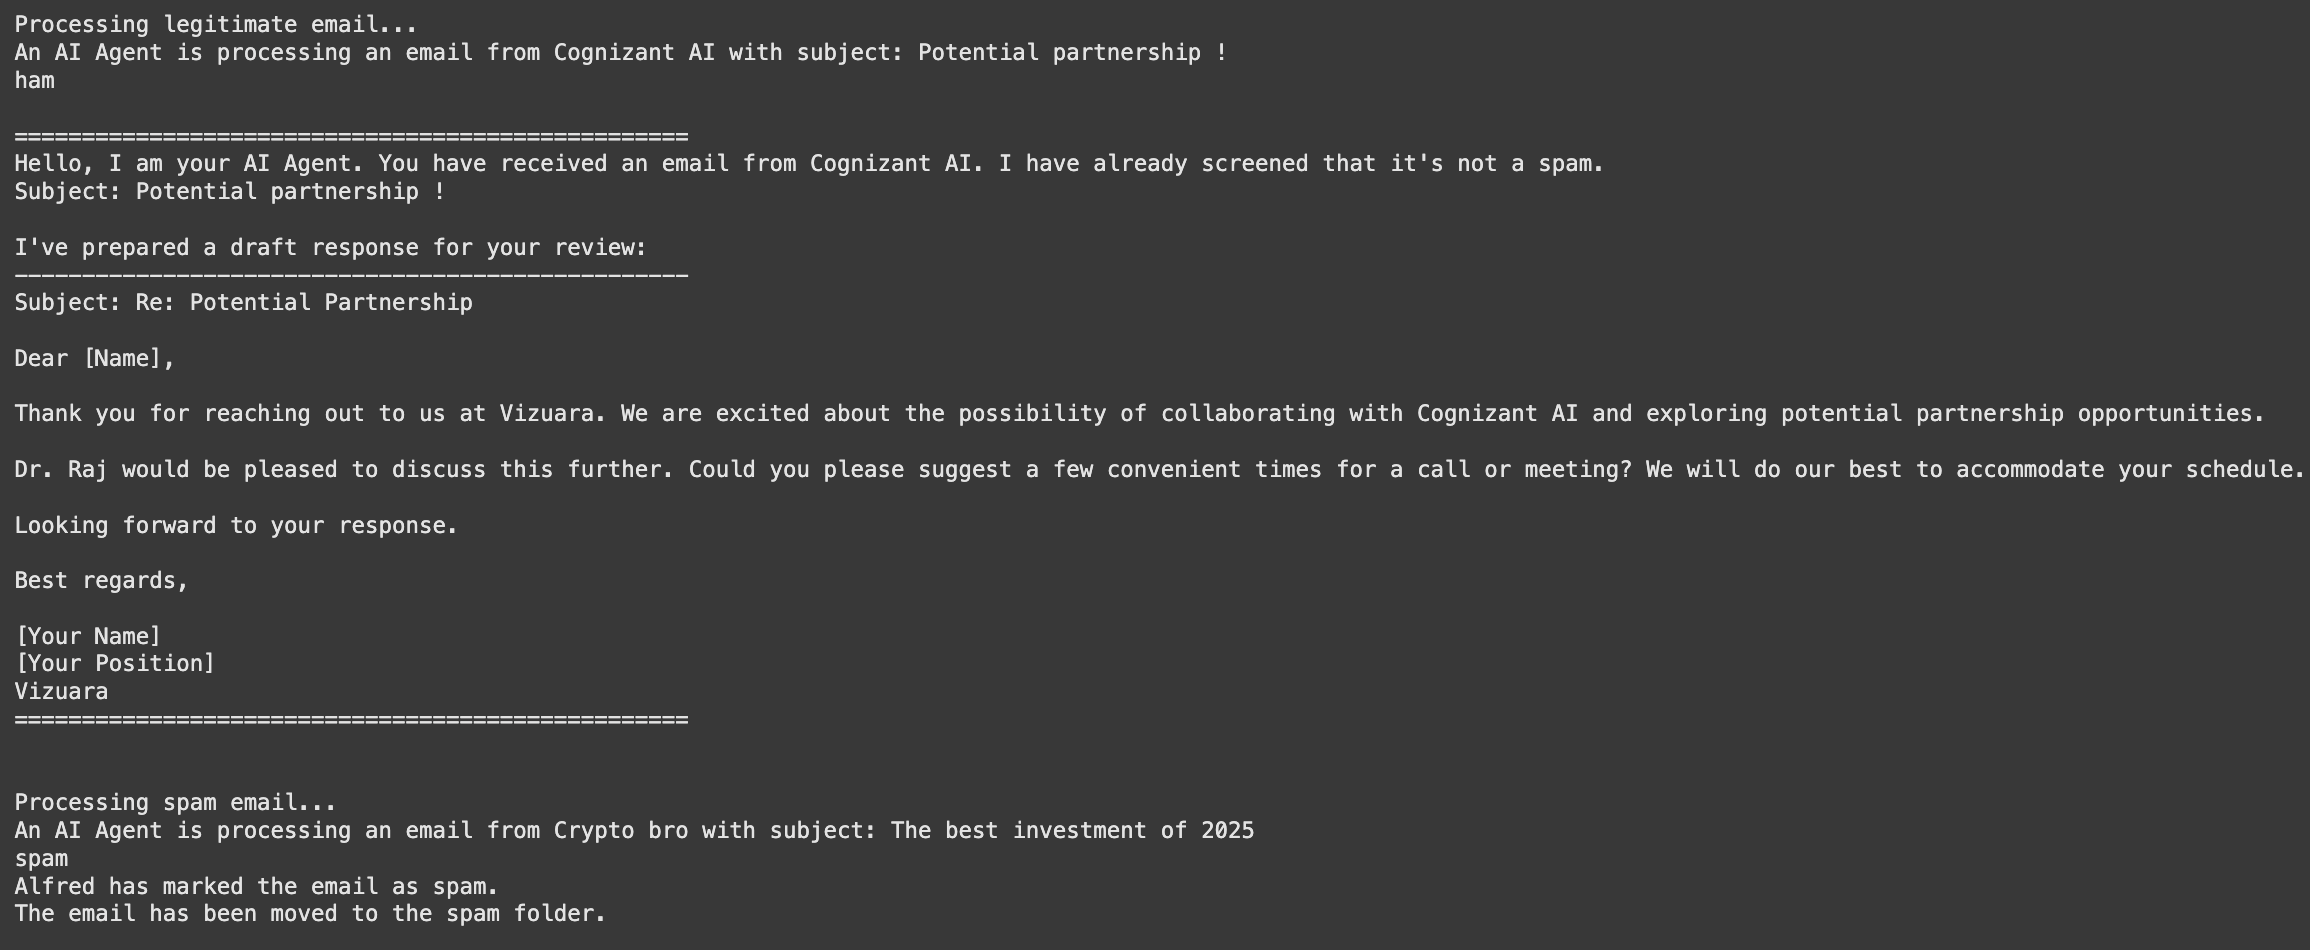
\includegraphics[width=\linewidth,keepaspectratio]{aiagents75}
		
		{\tiny (Ref: Vizuara AI Agents Bootcamp)}
				
        \end{center}    

\end{frame}


%%%%%%%%%%%%%%%%%%%%%%%%%%%%%%%%%%%%%%%%%%%%%%%%%%%%%%%%%%%%%%%%%%%%%%%%%%%%%%%%%%
\begin{frame}\frametitle{Concepts}

\begin{itemize}
\item Model: Large Language Model that supports Function Calling
\item Tools: Actions taken by app, ie API calls, Db operations, etc
\item State: Represents info that is carried though out the workflow e.g Message State has list of messages produced from each Node.
\item Node: executable logic container, a Langchain runnable or a Tool invoker. Nodes are connected by edges.
\item Edge: control flow of info, conditional or normal
\item Workflow: The graph, having nodes and edges, can be invoked or streamed from.
\end{itemize}

\begin{center}
\includegraphics[width=0.8\linewidth,keepaspectratio]{langgraph2}
\end{center}	  

{\tiny (Ref: Introduction to LangGraph | Building an AI Generated Podcast - Prompt Circle AI)}
\end{frame}

%%%%%%%%%%%%%%%%%%%%%%%%%%%%%%%%%%%%%%%%%%%%%%%%%%%%%%%%%%%
\begin{frame}[fragile]\frametitle{Graph and State Machine Concepts}
      \begin{itemize}
        \item State: System's behavioral condition (hunger, sleep, temperature)
        \item Events: Actions that trigger state changes (feeding, soothing)
        \item Nodes: Decision-makers and executors in the workflow
        \item Baby care analogy: Mother decides, elders check, father executes
        \item State updates trigger continuous decision-making cycles
        \item Graph structure provides flexible workflow representation
        \item State machines enable dynamic routing based on conditions
        \item More intuitive than linear processing chains
      \end{itemize}
\end{frame}

%%%%%%%%%%%%%%%%%%%%%%%%%%%%%%%%%%%%%%%%%%%%%%%%%%%%%%%%%%%
\begin{frame}[fragile]\frametitle{LangGraph Core Features}
      \begin{itemize}
        \item Looping and branching capabilities with conditional statements
        \item State persistence with automatic save and restore functionality
        \item Human-machine interaction support with review and editing
        \item Streaming processing for real-time feedback and status updates
        \item Seamless integration with existing LangChain components
        \item Support for LCEL expressions and rich tool ecosystem
        \item Flexible interaction control mechanisms
        \item Enhanced user experience through responsive design
      \end{itemize}
\end{frame}

%%%%%%%%%%%%%%%%%%%%%%%%%%%%%%%%%%%%%%%%%%%%%%%%%%%%%%%%%%%
\begin{frame}[fragile]\frametitle{Core Concept: State}

      \begin{itemize}
        \item State is the foundation of LangGraph applications
        \item Can be simple dictionary or Pydantic model
        \item Contains all information needed during runtime
        \item Passed between nodes and updated throughout execution
      \end{itemize}
	  
      \begin{lstlisting}[language=Python, basicstyle=\small]
from typing import List, Dict
from pydantic import BaseModel

class ChatState(BaseModel):
    messages: List[Dict[str, str]] = []
    current_input: str = ""
    tools_output: Dict[str, str] = {}
    final_response: str = ""
      \end{lstlisting}

\end{frame}

%%%%%%%%%%%%%%%%%%%%%%%%%%%%%%%%%%%%%%%%%%%%%%%%%%%%%%%%%%%
\begin{frame}[fragile]\frametitle{Core Concept: Nodes}
      \begin{lstlisting}[language=Python, basicstyle=\small]
async def process_input(state: ChatState) -> ChatState:
    # Process user input
    messages = state.messages + [{"role": "user", "content": state.current_input}]
    return ChatState(
        messages=messages,
        current_input=state.current_input,
        tools_output=state.tools_output
    )

async def generate_response(state: ChatState) -> ChatState:
    # Generate response using LLM
    response = await llm.ainvoke(state.messages)
    messages = state.messages + [{"role": "assistant", "content": response}]
    return ChatState(
        messages=messages,
        current_input=state.current_input,
        tools_output=state.tools_output,
        final_response=response
    )
      \end{lstlisting}
\end{frame}

%%%%%%%%%%%%%%%%%%%%%%%%%%%%%%%%%%%%%%%%%%%%%%%%%%%%%%%%%%%
\begin{frame}[fragile]\frametitle{Core Concept: Edges}

      \begin{itemize}
        \item Edges define connections and routing logic between nodes
        \item Support conditional routing based on state
        \item Enable dynamic execution paths
      \end{itemize}
	  
      \begin{lstlisting}[language=Python, basicstyle=\small]
from langgraph.graph import StateGraph, END

# Create graph structure
workflow = StateGraph(ChatState)

# Add nodes
workflow.add_node("process_input", process_input)
workflow.add_node("generate_response", generate_response)

# Define edges and routing logic
workflow.add_edge("process_input", "generate_response")
workflow.add_edge("generate_response", END)
      \end{lstlisting}

\end{frame}

%%%%%%%%%%%%%%%%%%%%%%%%%%%%%%%%%%%%%%%%%%%%%%%%%%%%%%%%%%%
\begin{frame}[fragile]\frametitle{Simple Chatbot Implementation}
      \begin{lstlisting}[language=Python, basicstyle=\tiny]
from typing import List, Dict
from pydantic import BaseModel
from langgraph.graph import StateGraph, END
from langchain_core.language_models import ChatOpenAI

class ChatState(BaseModel):
    messages: List[Dict[str, str]] = []
    current_input: str = ""
    should_continue: bool = True

async def process_user_input(state: ChatState) -> ChatState:
    messages = state.messages + [{"role": "user", "content": state.current_input}]
    return ChatState(
        messages=messages,
        current_input=state.current_input,
        should_continue=True
    )

async def generate_ai_response(state: ChatState) -> ChatState:
    llm = ChatOpenAI(temperature=0.7)
    response = await llm.ainvoke(state.messages)
    messages = state.messages + [{"role": "assistant", "content": response}]
    return ChatState(
        messages=messages,
        current_input=state.current_input,
        should_continue=True
    )

def should_continue(state: ChatState) -> str:
    if "goodbye" in state.current_input.lower():
        return "end"
    return "continue"
      \end{lstlisting}
\end{frame}

%%%%%%%%%%%%%%%%%%%%%%%%%%%%%%%%%%%%%%%%%%%%%%%%%%%%%%%%%%%
\begin{frame}[fragile]\frametitle{Building the Chatbot Graph}
      \begin{lstlisting}[language=Python, basicstyle=\tiny]
# Build the graph
workflow = StateGraph(ChatState)

# Add nodes
workflow.add_node("process_input", process_user_input)
workflow.add_node("generate_response", generate_ai_response)

# Add edges
workflow.add_edge("process_input", "generate_response")
workflow.add_conditional_edges("generate_response", should_continue, 
    {"continue": "process_input", "end": END})

# Compile the graph
app = workflow.compile()

# Run the conversation
async def chat():
    state = ChatState()
    while True:
        user_input = input("You: ")
        state.current_input = user_input
        state = await app.ainvoke(state)
        print("Bot:", state.messages[-1]["content"])
        if not state.should_continue:
            break
      \end{lstlisting}
\end{frame}

%%%%%%%%%%%%%%%%%%%%%%%%%%%%%%%%%%%%%%%%%%%%%%%%%%%%%%%%%%%
\begin{frame}[fragile]\frametitle{Advanced Conditional Edges}
      \begin{lstlisting}[language=Python, basicstyle=\tiny]
from typing import List, Dict, Literal
from pydantic import BaseModel

class AgentState(BaseModel):
    messages: List[Dict[str, str]] = []
    current_input: str = ""
    tools_output: Dict[str, str] = {}
    status: str = "RUNNING"
    error_count: int = 0

def route_by_status(state: AgentState) -> Literal["process", "retry", "error", "end"]:
    if state.status == "SUCCESS":
        return "end"
    elif state.status == "ERROR":
        if state.error_count >= 3:
            return "error"
        return "retry"
    elif state.status == "NEED_TOOL":
        return "process"
    return "process"

workflow.add_conditional_edges(
    "check_status",
    route_by_status,
    {"process": "execute_tool", "retry": "retry_handler", 
     "error": "error_handler", "end": END}
)
      \end{lstlisting}
\end{frame}

%%%%%%%%%%%%%%%%%%%%%%%%%%%%%%%%%%%%%%%%%%%%%%%%%%%%%%%%%%%
\begin{frame}[fragile]\frametitle{Parallel Execution in LangGraph}
      \begin{lstlisting}[language=Python, basicstyle=\tiny]
async def parallel_tools_execution(state: AgentState) -> AgentState:
    """Parallel execution of multiple tools"""
    tools = identify_required_tools(state.current_input)

    async def execute_tool(tool):
        result = await tool.ainvoke(state.current_input)
        return {tool.name: result}

    # Execute all tools in parallel
    results = await asyncio.gather(*[execute_tool(tool) for tool in tools])

    # Merge results
    tools_output = {}
    for result in results:
        tools_output.update(result)

    return AgentState(
        messages=state.messages,
        current_input=state.current_input,
        tools_output=tools_output,
        status="SUCCESS"
    )
      \end{lstlisting}
\end{frame}

%%%%%%%%%%%%%%%%%%%%%%%%%%%%%%%%%%%%%%%%%%%%%%%%%%%%%%%%%%%
\begin{frame}[fragile]\frametitle{ReACT Architecture Introduction}
      \begin{itemize}
        \item ReACT (Reasoning and Acting) combines reasoning and acting capabilities
        \item Agent solves problems through continuous cycle: Reason → Act → Observe
        \item Flexible response to complex tasks using external tools
        \item Enhanced capabilities through tool integration
        \item LangGraph provides pre-built ReACT agents
        \item Supports Google search, DALL-E image generation, and more
        \item Easy implementation with create\_react\_agent function
        \item Suitable for dynamic problem-solving scenarios
      \end{itemize}
\end{frame}

%%%%%%%%%%%%%%%%%%%%%%%%%%%%%%%%%%%%%%%%%%%%%%%%%%%%%%%%%%%
\begin{frame}[fragile]\frametitle{ReACT Agent Implementation}
      \begin{lstlisting}[language=Python, basicstyle=\tiny]
import dotenv
from langchain_community.tools import GoogleSerperRun
from langchain_community.tools.openai_dalle_image_generation import OpenAIDALLEImageGenerationTool
from langchain_openai import ChatOpenAI
from langgraph.prebuilt.chat_agent_executor import create_react_agent

dotenv.load_dotenv()

# Define tools
google_serper = GoogleSerperRun(
    name="google_serper",
    description="A low-cost Google search API for current events",
    args_schema=GoogleSerperArgsSchema,
    api_wrapper=GoogleSerperAPIWrapper(),
)

dalle = OpenAIDALLEImageGenerationTool(
    name="openai_dalle",
    api_wrapper=DallEAPIWrapper(model="dall-e-3"),
    args_schema=DallEArgsSchema,
)

tools = [google_serper, dalle]
model = ChatOpenAI(model="gpt-4o-mini", temperature=0)

# Create ReACT agent
agent = create_react_agent(model=model, tools=tools)

# Usage
result = agent.invoke({"messages": [("human", "Help me draw a shark flying in the sky")]})
      \end{lstlisting}
\end{frame}

%%%%%%%%%%%%%%%%%%%%%%%%%%%%%%%%%%%%%%%%%%%%%%%%%%%%%%%%%%%
\begin{frame}[fragile]\frametitle{Message Management in LangGraph}
      \begin{itemize}
        \item Message accumulation can lead to performance issues
        \item delete\_messages function removes processed messages
        \item Filtering techniques control message flow
        \item Conditional edges for message routing
        \item Time-based and quantity-based pruning strategies
        \item Essential for long-running applications
        \item Maintains conversation clarity and focus
        \item Improves overall system performance
      \end{itemize}
\end{frame}

%%%%%%%%%%%%%%%%%%%%%%%%%%%%%%%%%%%%%%%%%%%%%%%%%%%%%%%%%%%
\begin{frame}[fragile]\frametitle{Message Deletion and Filtering}
      \begin{lstlisting}[language=Python, basicstyle=\tiny]
from langgraph.prebuilt import ToolMessage, delete_messages

def process_and_delete(state):
    # Processing logic
    # Delete processed messages
    state = delete_messages(state, lambda x: isinstance(x, ToolMessage))
    return state

def filter_messages(state):
    filtered_messages = [msg for msg in state['messages'] 
                        if not isinstance(msg, ToolMessage)]
    return {"messages": filtered_messages}

def keep_latest_messages(state, max_messages=50):
    return {"messages": state['messages'][-max_messages:]}

# Time-based pruning
from datetime import datetime, timedelta

def prune_old_messages(state):
    current_time = datetime.now()
    recent_messages = [msg for msg in state['messages'] 
                      if current_time - msg.timestamp < timedelta(hours=1)]
    return {"messages": recent_messages}
      \end{lstlisting}
\end{frame}

%%%%%%%%%%%%%%%%%%%%%%%%%%%%%%%%%%%%%%%%%%%%%%%%%%%%%%%%%%%
\begin{frame}[fragile]\frametitle{Checkpoint Mechanism}
      \begin{itemize}
        \item Checkpoints are snapshots during graph execution
        \item Enable pause and resume functionality for long-running tasks
        \item Useful for processes requiring human intervention
        \item Support state rollback to previous points
        \item Allow data modification at checkpoints
        \item Use thread\_id and thread\_ts for unique identification
        \item Retrieve last state and execution history
        \item Essential for resumable AI applications
      \end{itemize}
\end{frame}

%%%%%%%%%%%%%%%%%%%%%%%%%%%%%%%%%%%%%%%%%%%%%%%%%%%%%%%%%%%
\begin{frame}[fragile]\frametitle{Checkpoint Implementation}
      \begin{lstlisting}[language=Python, basicstyle=\tiny]
from langgraph.checkpoint import create_checkpoint, load_checkpoint

def process_with_checkpoint(state):
    # Processing logic
    # Create a checkpoint
    checkpoint = create_checkpoint(state)
    return {"checkpoint": checkpoint, "state": state}

def resume_from_checkpoint(checkpoint):
    state = load_checkpoint(checkpoint)
    # Continue processing
    return state

# Using checkpoints in practice
def summarize_and_prune(state):
    summary = summarize_conversation(state['messages'])
    new_messages = state['messages'][-5:]
    new_messages.append(ToolMessage(content=summary))
    state['messages'] = new_messages
    
    # Create checkpoint
    checkpoint = create_checkpoint(state)
    state['checkpoint'] = checkpoint
    return state

# Retrieve state and history
graph.get_state(config)  # Get last saved state
graph.get_state_history(config)  # Get all saved states
      \end{lstlisting}
\end{frame}

%%%%%%%%%%%%%%%%%%%%%%%%%%%%%%%%%%%%%%%%%%%%%%%%%%%%%%%%%%%
\begin{frame}[fragile]\frametitle{Human-in-the-Loop Interaction}
      \begin{itemize}
        \item Allows human participation in AI decision-making process
        \item Callback functions obtain human input during execution
        \item Conditional branching determines when human intervention needed
        \item Confidence-based routing for automatic vs manual processing
        \item Enhanced system reliability through human oversight
        \item Flexible interaction control mechanisms
        \item Improves decision quality in critical scenarios
        \item Supports collaborative human-AI workflows
      \end{itemize}
\end{frame}

%%%%%%%%%%%%%%%%%%%%%%%%%%%%%%%%%%%%%%%%%%%%%%%%%%%%%%%%%%%
\begin{frame}[fragile]\frametitle{Human Interaction Implementation}
      \begin{lstlisting}[language=Python, basicstyle=\tiny]
def human_input_node(state):
    # Display current state to user
    print("Current state:", state)
    # Get user input
    user_input = input("Please provide your input: ")
    # Update state
    state['user_input'] = user_input
    return state

def check_confidence(state):
    if state['confidence'] < 0.8:
        return "human_input"
    else:
        return "auto_process"

def human_intervention(state):
    print("Current conversation:", state['messages'])
    human_response = input("Please provide assistance: ")
    state['messages'].append(HumanMessage(content=human_response))
    return state

# Add conditional routing
graph.add_conditional_edges("process_query", {
    "human_intervention": lambda s: s['confidence'] < 0.8,
    "auto_process": lambda s: s['confidence'] >= 0.8
})
      \end{lstlisting}
\end{frame}

%%%%%%%%%%%%%%%%%%%%%%%%%%%%%%%%%%%%%%%%%%%%%%%%%%%%%%%%%%%
\begin{frame}[fragile]\frametitle{Subgraph Architecture}
      \begin{itemize}
        \item Break complex workflows into manageable components
        \item Modular design enhances code reusability
        \item Independent subgraphs improve maintainability
        \item Easy testing and debugging of individual components
        \item Scalable architecture for adding new features
        \item Encapsulate complex logic in reusable modules
        \item Support composition and interaction between subgraphs
        \item Enable hierarchical workflow organization
      \end{itemize}
\end{frame}

%%%%%%%%%%%%%%%%%%%%%%%%%%%%%%%%%%%%%%%%%%%%%%%%%%%%%%%%%%%
\begin{frame}[fragile]\frametitle{Subgraph Implementation}
      \begin{lstlisting}[language=Python, basicstyle=\tiny]
from langgraph.graph import SubGraph, Graph

class ContentGenerationSubGraph(SubGraph):
    def build(self) -> Graph:
        graph = Graph()
        
        def generate_content(state):
            # Content generation logic
            return state
            
        def review_content(state):
            # Content review logic
            return state
            
        graph.add_node("generate_content", self.generate_content)
        graph.add_node("review_content", self.review_content)
        graph.add_edge("generate_content", "review_content")
        return graph

# Using subgraphs in main graph
def create_marketing_workflow():
    main_graph = Graph()
    content_graph = ContentGenerationSubGraph()
    analytics_graph = AnalyticsSubGraph()
    
    main_graph.add_node("content", content_graph)
    main_graph.add_node("analytics", analytics_graph)
    main_graph.add_edge("content", "analytics")
    return main_graph
      \end{lstlisting}
\end{frame}

%%%%%%%%%%%%%%%%%%%%%%%%%%%%%%%%%%%%%%%%%%%%%%%%%%%%%%%%%%%
\begin{frame}[fragile]\frametitle{Data State and Induction Functions}
      \begin{itemize}
        \item Default behavior overwrites original data completely
        \item Manual state retrieval and update prevents data loss
        \item Induction functions provide automatic data accumulation
        \item Annotated wrapper simplifies state management
        \item Independent node execution without state conflicts
        \item Type hints improve code clarity and debugging
        \item Simplified node modification when updating structures
        \item Enhanced data consistency across workflow execution
      \end{itemize}
\end{frame}

%%%%%%%%%%%%%%%%%%%%%%%%%%%%%%%%%%%%%%%%%%%%%%%%%%%%%%%%%%%
\begin{frame}[fragile]\frametitle{Induction Functions Example}
      \begin{lstlisting}[language=Python, basicstyle=\tiny]
from typing import TypedDict, Annotated

# Problem: Default behavior overwrites data
class MyState(TypedDict):
    messages: list

def fn1(state: MyState):
    return {"messages": [4]}

r = graph.invoke({"messages": [1, 2, 3]})
# Result: {"messages": [4]} instead of [1,2,3,4]

# Solution: Use induction functions
def concat_lists(original: list, new: list) -> list:
    return original + new

class MyState(TypedDict):
    messages: Annotated[list, concat_lists]

def fn1(state: MyState):
    return {"messages": [4]}

r = graph.invoke({"messages": [1, 2, 3]})
# Result: {'messages': [1, 2, 3, 4]}
      \end{lstlisting}
\end{frame}

%%%%%%%%%%%%%%%%%%%%%%%%%%%%%%%%%%%%%%%%%%%%%%%%%%%%%%%%%%%
\begin{frame}[fragile]\frametitle{Parallel Node Execution}
      \begin{itemize}
        \item END node signifies route termination, not graph termination
        \item Nodes at same level execute in parallel
        \item Execution order is uncertain in parallel execution
        \item Control flow by adjusting node connections
        \item Important for understanding graph execution model
        \item Optimize performance through parallel processing
        \item Design considerations for concurrent operations
        \item Manage dependencies between parallel nodes
      \end{itemize}
\end{frame}

%%%%%%%%%%%%%%%%%%%%%%%%%%%%%%%%%%%%%%%%%%%%%%%%%%%%%%%%%%%
\begin{frame}[fragile]\frametitle{Streaming Response in LangGraph}
      \begin{itemize}
        \item Different from traditional LLM word-by-word output
        \item Outputs node data state each time for granular control
        \item Values mode returns complete graph state (total)
        \item Updates mode returns state changes only (incremental)
        \item Compiled graph is essentially a Runnable component
        \item Multiple streaming modes for different use cases
        \item Enhanced user experience through real-time feedback
        \item Future improvements for node-level streaming
      \end{itemize}
\end{frame}

%%%%%%%%%%%%%%%%%%%%%%%%%%%%%%%%%%%%%%%%%%%%%%%%%%%%%%%%%%%
\begin{frame}[fragile]\frametitle{Streaming Modes Implementation}
      \begin{itemize}
        \item Values mode: Complete state after each node
        \item Updates mode: Incremental changes as dictionary
        \item Dictionary keys represent node names
        \item Dictionary values contain state updates
        \item Choose mode based on application requirements
      \end{itemize}
      \begin{lstlisting}[language=Python, basicstyle=\small]
# Values mode: Returns complete state values
inputs = {"messages": [("human", "What are the top 3 results of the 2024 Beijing Half Marathon?")]}

for chunk in agent.stream(inputs, stream_mode="values"):
    print(chunk["messages"][-1].pretty_print())

# Updates mode: Returns state updates only
for chunk in agent.stream(inputs, stream_mode="updates"):
    print(chunk)
      \end{lstlisting}

\end{frame}


%%%%%%%%%%%%%%%%%%%%%%%%%%%%%%%%%%%%%%%%%%%%%%%%%%%%%%%%%%%%%%%%%%%%%%%%%%%%%%%%%%
\begin{frame}[fragile]\frametitle{}
\begin{center}
{\Large Applications}
\end{center}
\end{frame}


%%%%%%%%%%%%%%%%%%%%%%%%%%%%%%%%%%%%%%%%%%%%%%%%%%%%%%%%%%%%%%%%%%%%%%%%%%%%%%%%%%
\begin{frame}\frametitle{Podcast Generator}

\begin{center}
\includegraphics[width=0.8\linewidth,keepaspectratio]{langgraph3}
\end{center}	  


{\tiny (Ref: Introduction to LangGraph | Building an AI Generated Podcast - Prompt Circle AI)}

Code at https://github.com/hollaugo/langgraph-framework-tutorial
\end{frame}


%%%%%%%%%%%%%%%%%%%%%%%%%%%%%%%%%%%%%%%%%%%%%%%%%%%%%%%%%%%%%%%%%%%%%%%%%%%%%%%%%%
\begin{frame}[fragile]\frametitle{News Aggregator}

\begin{center}
\includegraphics[width=0.8\linewidth,keepaspectratio]{langgraph4}
\end{center}	

Code: https://github.com/rajib76/multi\_agent/blob/main/01\_how\_to\_langgraph\_example\_01.py

{\tiny (Ref: Langgraph: The Agent Orchestrator - Rajib Deb)}


\end{frame}

%%%%%%%%%%%%%%%%%%%%%%%%%%%%%%%%%%%%%%%%%%%%%%%%%%%%%%%%%%%%%%%%%%%%%%%%%%%%%%%%%%
\begin{frame}[fragile]\frametitle{}
\begin{center}
{\Large Agents using LangGraph}
\end{center}
\end{frame}

%%%%%%%%%%%%%%%%%%%%%%%%%%%%%%%%%%%%%%%%%%%%%%%%%%%%%%%%%%%
\begin{frame}[fragile]\frametitle{Creating a Vision Assistant Agent}
\begin{columns}
    \begin{column}[T]{0.7\linewidth}
      \begin{itemize}
        \item Vision-enabled agent implementing explicit "Thought → Action → Observation" loop
        \item \textbf{AgentState:} Stores input\_file (image path) and messages list for conversation history
        \item \textbf{Assistant node:} GPT-4 with vision capability bound to image analysis and math tools
        \item \textbf{Tools node:} Executes tool functions (extract\_text, divide) and records results
        \item Assistant decides to use tools or provide final answer based on task requirements
        \item Conditional edge uses tools\_condition to route between assistant and tools nodes
        \item Creates cycle: assistant thinks → tool execution → assistant processes results → repeat
        \item Loop continues until assistant provides final answer without requesting tools
      \end{itemize}
    \end{column}
    \begin{column}[T]{0.3\linewidth}
        \begin{center}
        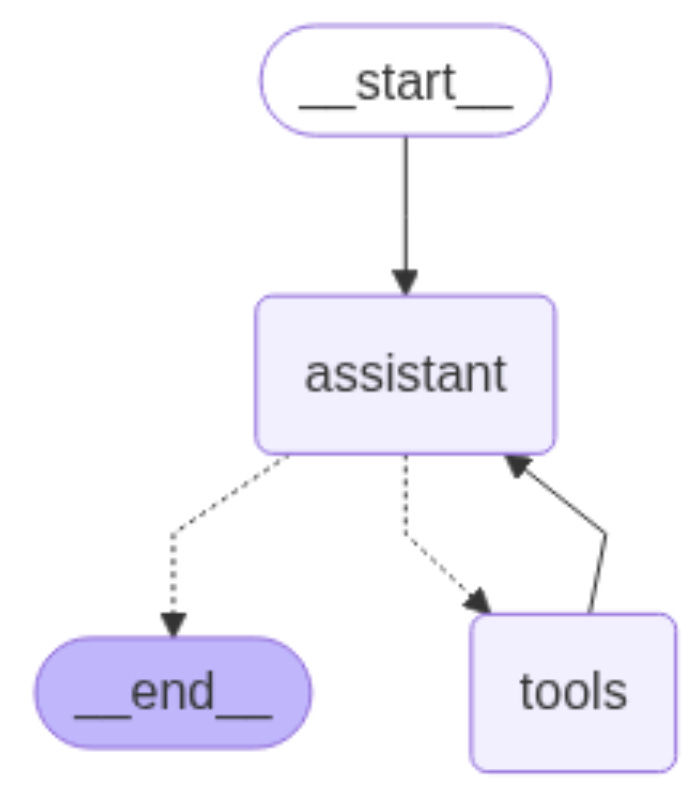
\includegraphics[width=\linewidth,keepaspectratio]{aiagents76}
        \end{center}    
    \end{column}
  \end{columns}
\end{frame}

%%%%%%%%%%%%%%%%%%%%%%%%%%%%%%%%%%%%%%%%%%%%%%%%%%%%%%%%%%%
\begin{frame}[fragile]\frametitle{Creating a Vision Assistant Agent}

        \begin{center}

        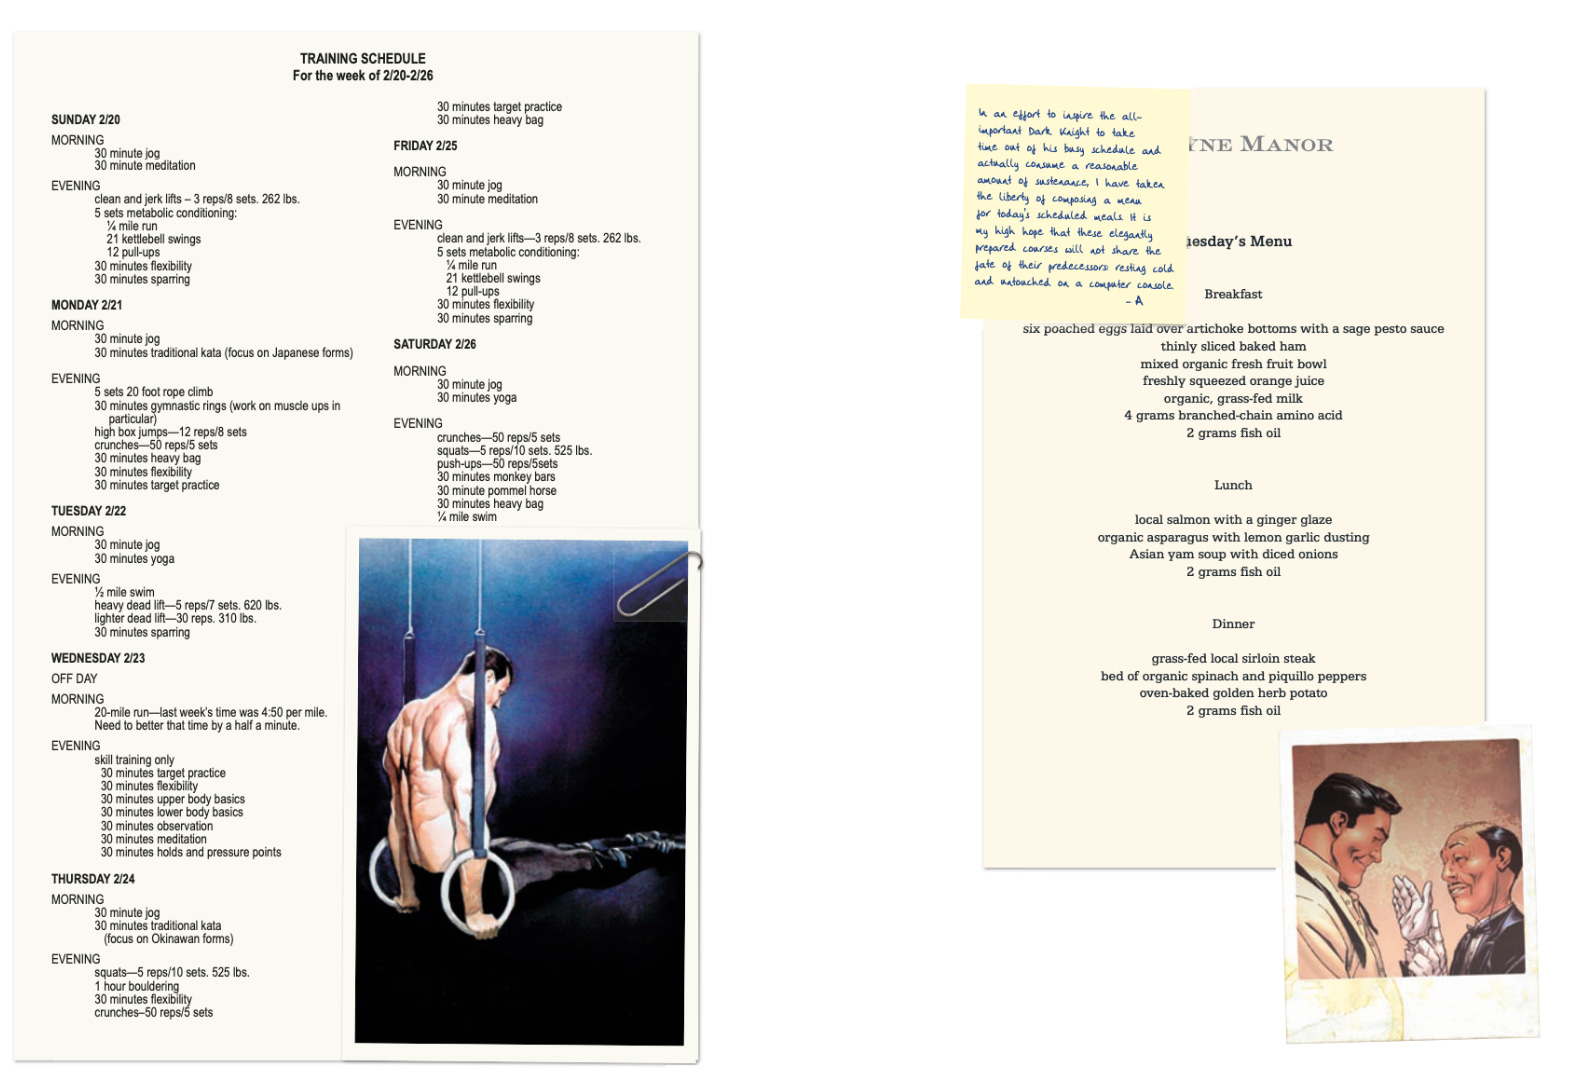
\includegraphics[width=0.9\linewidth,keepaspectratio]{aiagents77}
		
		{\tiny (Ref: Vizuara AI Agents Bootcamp)}
				
        \end{center}    

\end{frame}

%%%%%%%%%%%%%%%%%%%%%%%%%%%%%%%%%%%%%%%%%%%%%%%%%%%%%%%%%%%
\begin{frame}[fragile]\frametitle{Creating a Vision Assistant Agent}

        \begin{center}

        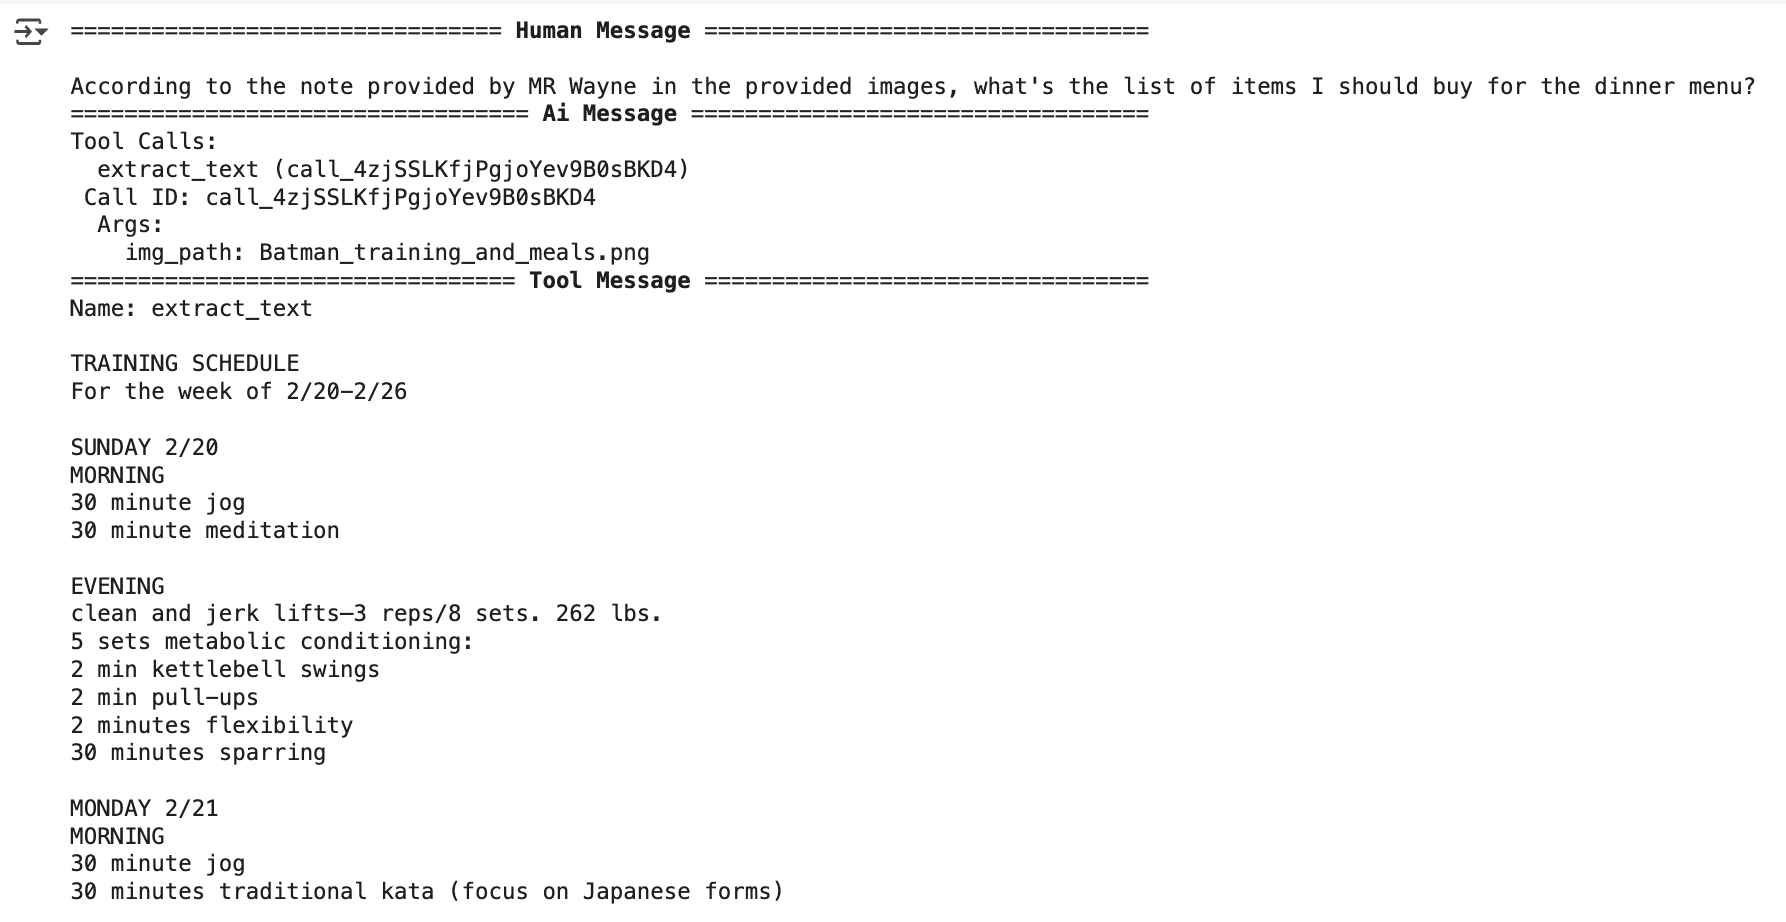
\includegraphics[width=\linewidth,keepaspectratio]{aiagents78}
		
		{\tiny (Ref: Vizuara AI Agents Bootcamp)}
				
        \end{center}    

\end{frame}



%%%%%%%%%%%%%%%%%%%%%%%%%%%%%%%%%%%%%%%%%%%%%%%%%%%%%%%%%%%
\begin{frame}[fragile]\frametitle{Tracing Agent Workflows with Langfuse}

      \begin{itemize}
        \item Observability crucial for debugging complex agent behaviors with multiple steps
        \item \textbf{Traces:} Detailed execution records capturing prompts, responses, paths, and tool usage
        \item Langfuse provides user-friendly dashboard for inspecting agent workflow traces
        \item Integrates via OpenTelemetry standards with tracing callbacks in LangGraph code
        \item Enables monitoring of both email agent and vision agent execution flows
        \item Tools-assistant loop clearly visible in Langfuse trace visualization
        \item Answers "why did my agent do X?" through accessible trace inspection
        \item Essential best practice for moving from prototypes to production-grade AI systems
      \end{itemize}

\end{frame}

%%%%%%%%%%%%%%%%%%%%%%%%%%%%%%%%%%%%%%%%%%%%%%%%%%%%%%%%%%%
\begin{frame}[fragile]\frametitle{Tracing Agent Workflows with Langfuse}

        \begin{center}

        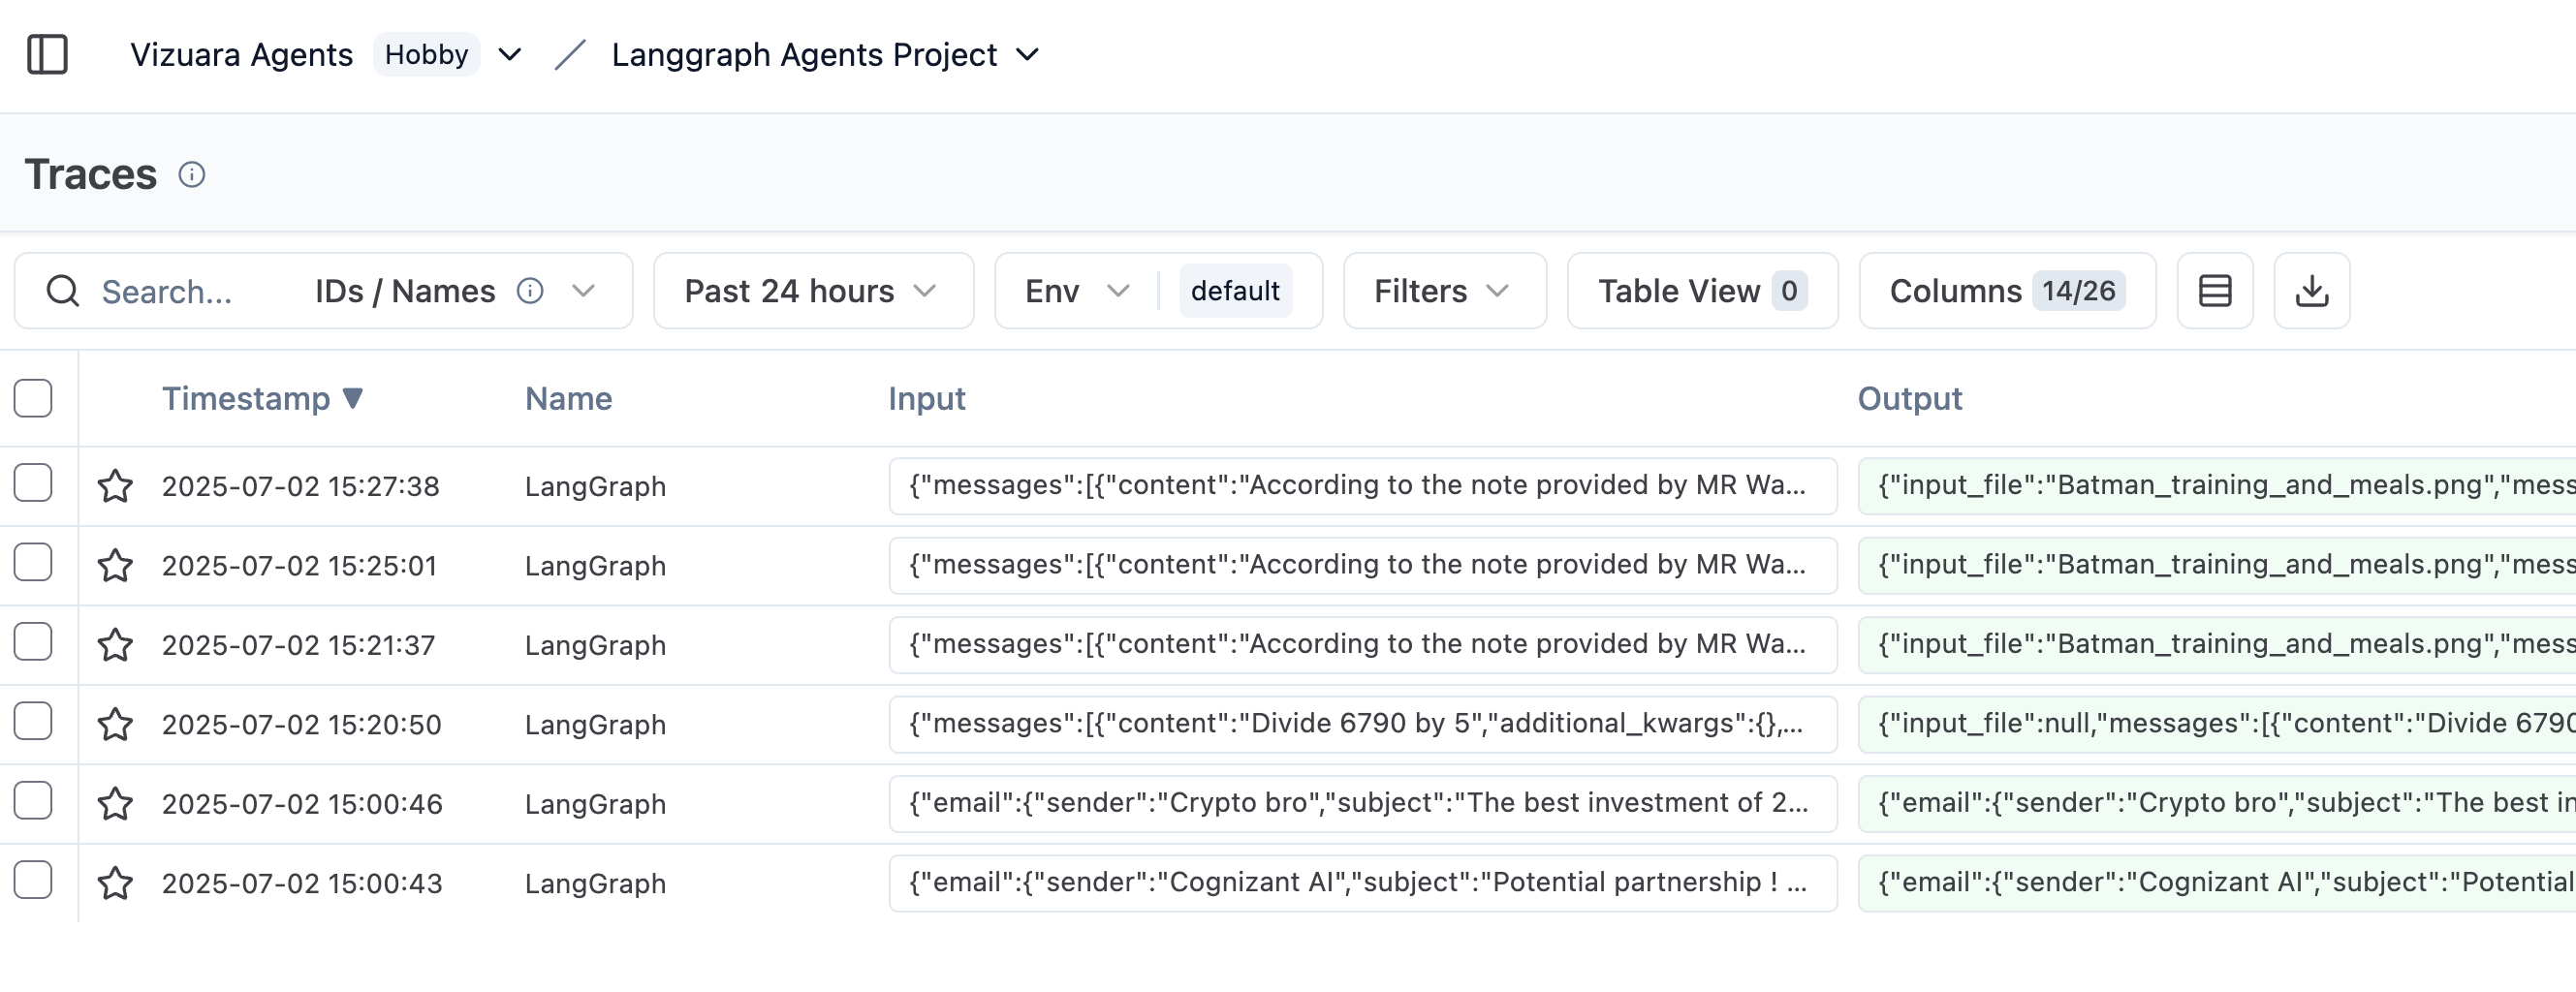
\includegraphics[width=\linewidth,keepaspectratio]{aiagents79}
		
		{\tiny (Ref: Vizuara AI Agents Bootcamp)}
				
        \end{center}    

\end{frame}

%%%%%%%%%%%%%%%%%%%%%%%%%%%%%%%%%%%%%%%%%%%%%%%%%%%%%%%%%%%
\begin{frame}[fragile]\frametitle{Tracing Agent Workflows with Langfuse}

        \begin{center}

        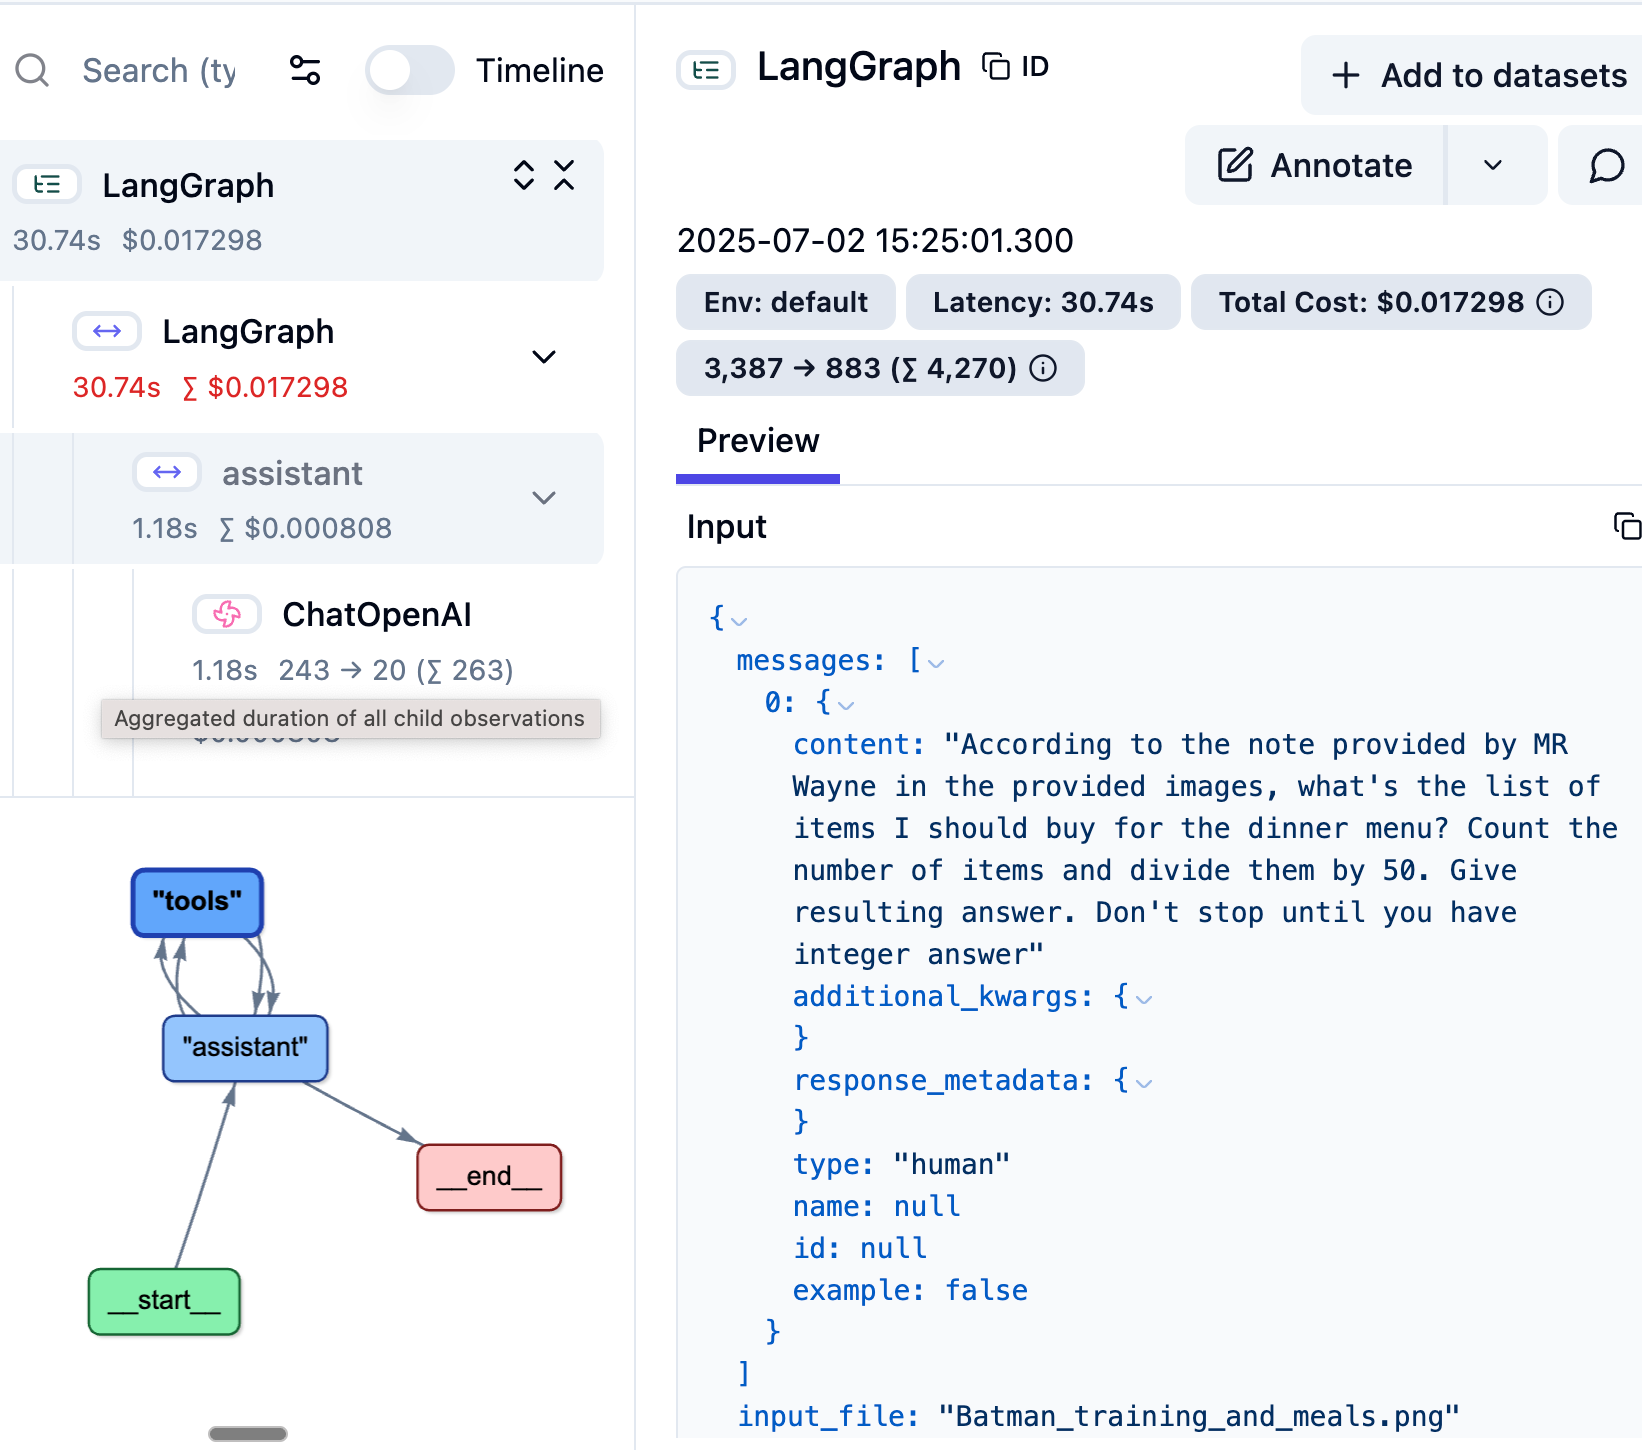
\includegraphics[width=0.7\linewidth,keepaspectratio]{aiagents80}
		
		{\tiny (Ref: Vizuara AI Agents Bootcamp)}
				
        \end{center}    

\end{frame}


%%%%%%%%%%%%%%%%%%%%%%%%%%%%%%%%%%%%%%%%%%%%%%%%%%%%%%%%%%%
\begin{frame}[fragile]\frametitle{Best Practices and Considerations}
      \begin{itemize}
        \item Keep state models simple and clear with necessary information only
        \item Maintain single responsibility in node functions
        \item Handle exceptions and return new state objects
        \item Use clear conditional logic in edge design
        \item Avoid complex cyclic dependencies in workflow
        \item Add error handling at critical nodes with fallback mechanisms
        \item Consider performance impacts of checkpoint mechanism
        \item Choose appropriate data processing methods for use cases
      \end{itemize}
\end{frame}

%%%%%%%%%%%%%%%%%%%%%%%%%%%%%%%%%%%%%%%%%%%%%%%%%%%%%%%%%%%
\begin{frame}[fragile]\frametitle{Future Developments and Limitations}
      \begin{itemize}
        \item Current streaming has long waiting times for LLM nodes
        \item Ideal: Node-level streaming within graph streaming
        \item Market agents provide better step-by-step streaming
        \item LangGraph rapidly evolving with frequent updates
        \item Pre-built components may change in future versions
        \item Monitor documentation for latest features and changes
        \item Core design philosophy remains valuable for learning
        \item Expected improvements in streaming processing capabilities
      \end{itemize}
\end{frame}

%%%%%%%%%%%%%%%%%%%%%%%%%%%%%%%%%%%%%%%%%%%%%%%%%%%%%%%%%%%
\begin{frame}[fragile]\frametitle{Conclusion}
      \begin{itemize}
        \item LangGraph addresses LCEL and AgentExecutor limitations effectively
        \item Graph-based approach provides intuitive workflow representation
        \item Advanced features support complex AI application development
        \item State management and persistence enable long-running conversations
        \item Human-in-the-loop capabilities enhance decision quality
        \item Modular subgraph architecture improves maintainability
        \item Streaming responses provide real-time user feedback
        \item Continuous evolution promises enhanced capabilities for AI development
      \end{itemize}
\end{frame}